% Created by tikzDevice version 0.12.4 on 2023-03-21 21:49:41
% !TEX encoding = UTF-8 Unicode
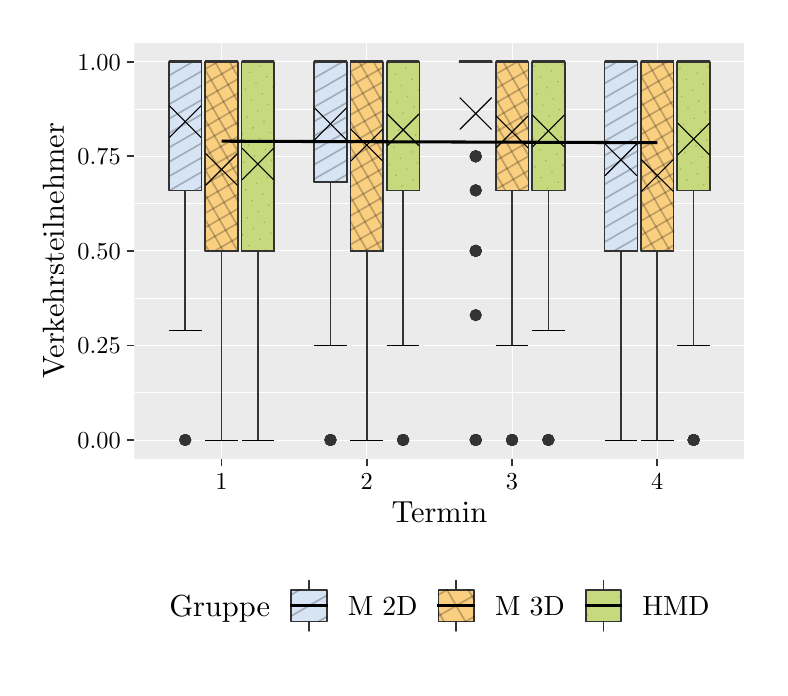
\begin{tikzpicture}[x=1pt,y=1pt]
\definecolor{fillColor}{RGB}{255,255,255}
\path[use as bounding box,fill=fillColor,fill opacity=0.00] (0,0) rectangle (264.51,231.26);
\begin{scope}
\path[clip] (  0.00,  0.00) rectangle (264.51,231.26);
\definecolor{drawColor}{RGB}{255,255,255}
\definecolor{fillColor}{RGB}{255,255,255}

\path[draw=drawColor,line width= 0.6pt,line join=round,line cap=round,fill=fillColor] (  0.00, -0.00) rectangle (264.51,231.26);
\end{scope}
\begin{scope}
\path[clip] ( 38.56, 75.45) rectangle (259.01,225.76);
\definecolor{fillColor}{gray}{0.92}

\path[fill=fillColor] ( 38.56, 75.45) rectangle (259.01,225.76);
\definecolor{drawColor}{RGB}{255,255,255}

\path[draw=drawColor,line width= 0.3pt,line join=round] ( 38.56, 99.36) --
	(259.01, 99.36);

\path[draw=drawColor,line width= 0.3pt,line join=round] ( 38.56,133.52) --
	(259.01,133.52);

\path[draw=drawColor,line width= 0.3pt,line join=round] ( 38.56,167.69) --
	(259.01,167.69);

\path[draw=drawColor,line width= 0.3pt,line join=round] ( 38.56,201.85) --
	(259.01,201.85);

\path[draw=drawColor,line width= 0.3pt,line join=round] ( 38.56, 82.28) --
	(259.01, 82.28);

\path[draw=drawColor,line width= 0.3pt,line join=round] ( 38.56,116.44) --
	(259.01,116.44);

\path[draw=drawColor,line width= 0.3pt,line join=round] ( 38.56,150.61) --
	(259.01,150.61);

\path[draw=drawColor,line width= 0.3pt,line join=round] ( 38.56,184.77) --
	(259.01,184.77);

\path[draw=drawColor,line width= 0.3pt,line join=round] ( 38.56,218.93) --
	(259.01,218.93);

\path[draw=drawColor,line width= 0.3pt,line join=round] ( 70.05, 75.45) --
	( 70.05,225.76);

\path[draw=drawColor,line width= 0.3pt,line join=round] (122.54, 75.45) --
	(122.54,225.76);

\path[draw=drawColor,line width= 0.3pt,line join=round] (175.03, 75.45) --
	(175.03,225.76);

\path[draw=drawColor,line width= 0.3pt,line join=round] (227.51, 75.45) --
	(227.51,225.76);
\definecolor{drawColor}{RGB}{0,0,0}

\path[draw=drawColor,line width= 0.2pt,line join=round] ( 51.02,218.93) --
	( 62.83,218.93);

\path[draw=drawColor,line width= 0.2pt,line join=round] ( 56.93,218.93) --
	( 56.93,121.91);

\path[draw=drawColor,line width= 0.2pt,line join=round] ( 51.02,121.91) --
	( 62.83,121.91);

\path[draw=drawColor,line width= 0.2pt,line join=round] ( 64.14,218.93) --
	( 75.95,218.93);

\path[draw=drawColor,line width= 0.2pt,line join=round] ( 70.05,218.93) --
	( 70.05, 82.28);

\path[draw=drawColor,line width= 0.2pt,line join=round] ( 64.14, 82.28) --
	( 75.95, 82.28);

\path[draw=drawColor,line width= 0.2pt,line join=round] ( 77.27,218.93) --
	( 89.08,218.93);

\path[draw=drawColor,line width= 0.2pt,line join=round] ( 83.17,218.93) --
	( 83.17, 82.28);

\path[draw=drawColor,line width= 0.2pt,line join=round] ( 77.27, 82.28) --
	( 89.08, 82.28);

\path[draw=drawColor,line width= 0.2pt,line join=round] (103.51,218.93) --
	(115.32,218.93);

\path[draw=drawColor,line width= 0.2pt,line join=round] (109.41,218.93) --
	(109.41,116.44);

\path[draw=drawColor,line width= 0.2pt,line join=round] (103.51,116.44) --
	(115.32,116.44);

\path[draw=drawColor,line width= 0.2pt,line join=round] (116.63,218.93) --
	(128.44,218.93);

\path[draw=drawColor,line width= 0.2pt,line join=round] (122.54,218.93) --
	(122.54, 82.28);

\path[draw=drawColor,line width= 0.2pt,line join=round] (116.63, 82.28) --
	(128.44, 82.28);

\path[draw=drawColor,line width= 0.2pt,line join=round] (129.75,218.93) --
	(141.56,218.93);

\path[draw=drawColor,line width= 0.2pt,line join=round] (135.66,218.93) --
	(135.66,116.44);

\path[draw=drawColor,line width= 0.2pt,line join=round] (129.75,116.44) --
	(141.56,116.44);

\path[draw=drawColor,line width= 0.2pt,line join=round] (156.00,218.93) --
	(167.81,218.93);

\path[draw=drawColor,line width= 0.2pt,line join=round] (161.90,218.93) --
	(161.90,218.93);

\path[draw=drawColor,line width= 0.2pt,line join=round] (156.00,218.93) --
	(167.81,218.93);

\path[draw=drawColor,line width= 0.2pt,line join=round] (169.12,218.93) --
	(180.93,218.93);

\path[draw=drawColor,line width= 0.2pt,line join=round] (175.03,218.93) --
	(175.03,116.44);

\path[draw=drawColor,line width= 0.2pt,line join=round] (169.12,116.44) --
	(180.93,116.44);

\path[draw=drawColor,line width= 0.2pt,line join=round] (182.24,218.93) --
	(194.05,218.93);

\path[draw=drawColor,line width= 0.2pt,line join=round] (188.15,218.93) --
	(188.15,121.91);

\path[draw=drawColor,line width= 0.2pt,line join=round] (182.24,121.91) --
	(194.05,121.91);

\path[draw=drawColor,line width= 0.2pt,line join=round] (208.49,218.93) --
	(220.30,218.93);

\path[draw=drawColor,line width= 0.2pt,line join=round] (214.39,218.93) --
	(214.39, 82.28);

\path[draw=drawColor,line width= 0.2pt,line join=round] (208.49, 82.28) --
	(220.30, 82.28);

\path[draw=drawColor,line width= 0.2pt,line join=round] (221.61,218.93) --
	(233.42,218.93);

\path[draw=drawColor,line width= 0.2pt,line join=round] (227.51,218.93) --
	(227.51, 82.28);

\path[draw=drawColor,line width= 0.2pt,line join=round] (221.61, 82.28) --
	(233.42, 82.28);

\path[draw=drawColor,line width= 0.2pt,line join=round] (234.73,218.93) --
	(246.54,218.93);

\path[draw=drawColor,line width= 0.2pt,line join=round] (240.64,218.93) --
	(240.64,116.44);

\path[draw=drawColor,line width= 0.2pt,line join=round] (234.73,116.44) --
	(246.54,116.44);
\definecolor{drawColor}{gray}{0.20}
\definecolor{fillColor}{gray}{0.20}

\path[draw=drawColor,line width= 0.4pt,line join=round,line cap=round,fill=fillColor] ( 56.93, 82.28) circle (  1.96);

\path[draw=drawColor,line width= 0.4pt,line join=round,line cap=round,fill=fillColor] ( 56.93, 82.28) circle (  1.96);

\path[draw=drawColor,line width= 0.2pt,line join=round] ( 56.93,218.93) -- ( 56.93,218.93);

\path[draw=drawColor,line width= 0.2pt,line join=round] ( 56.93,172.47) -- ( 56.93,121.91);
\definecolor{fillColor}{RGB}{215,228,244}

\path[draw=drawColor,line width= 0.2pt,fill=fillColor] ( 51.02,218.93) --
	( 51.02,172.47) --
	( 62.83,172.47) --
	( 62.83,218.93) --
	( 51.02,218.93) --
	cycle;

\path[draw=drawColor,line width= 0.5pt] ( 51.02,218.93) -- ( 62.83,218.93);

\path[draw=drawColor,line width= 0.2pt,line join=round] ( 70.05,218.93) -- ( 70.05,218.93);

\path[draw=drawColor,line width= 0.2pt,line join=round] ( 70.05,150.61) -- ( 70.05, 82.28);
\definecolor{fillColor}{RGB}{250,208,128}

\path[draw=drawColor,line width= 0.2pt,fill=fillColor] ( 64.14,218.93) --
	( 64.14,150.61) --
	( 75.95,150.61) --
	( 75.95,218.93) --
	( 64.14,218.93) --
	cycle;

\path[draw=drawColor,line width= 0.5pt] ( 64.14,218.93) -- ( 75.95,218.93);

\path[draw=drawColor,line width= 0.2pt,line join=round] ( 83.17,218.93) -- ( 83.17,218.93);

\path[draw=drawColor,line width= 0.2pt,line join=round] ( 83.17,150.61) -- ( 83.17, 82.28);
\definecolor{fillColor}{RGB}{199,217,125}

\path[draw=drawColor,line width= 0.2pt,fill=fillColor] ( 77.27,218.93) --
	( 77.27,150.61) --
	( 89.08,150.61) --
	( 89.08,218.93) --
	( 77.27,218.93) --
	cycle;

\path[draw=drawColor,line width= 0.5pt] ( 77.27,218.93) -- ( 89.08,218.93);
\definecolor{fillColor}{gray}{0.20}

\path[draw=drawColor,line width= 0.4pt,line join=round,line cap=round,fill=fillColor] (109.41, 82.28) circle (  1.96);

\path[draw=drawColor,line width= 0.4pt,line join=round,line cap=round,fill=fillColor] (109.41, 82.28) circle (  1.96);

\path[draw=drawColor,line width= 0.4pt,line join=round,line cap=round,fill=fillColor] (109.41, 82.28) circle (  1.96);

\path[draw=drawColor,line width= 0.2pt,line join=round] (109.41,218.93) -- (109.41,218.93);

\path[draw=drawColor,line width= 0.2pt,line join=round] (109.41,175.54) -- (109.41,116.44);
\definecolor{fillColor}{RGB}{215,228,244}

\path[draw=drawColor,line width= 0.2pt,fill=fillColor] (103.51,218.93) --
	(103.51,175.54) --
	(115.32,175.54) --
	(115.32,218.93) --
	(103.51,218.93) --
	cycle;

\path[draw=drawColor,line width= 0.5pt] (103.51,218.93) -- (115.32,218.93);

\path[draw=drawColor,line width= 0.2pt,line join=round] (122.54,218.93) -- (122.54,218.93);

\path[draw=drawColor,line width= 0.2pt,line join=round] (122.54,150.61) -- (122.54, 82.28);
\definecolor{fillColor}{RGB}{250,208,128}

\path[draw=drawColor,line width= 0.2pt,fill=fillColor] (116.63,218.93) --
	(116.63,150.61) --
	(128.44,150.61) --
	(128.44,218.93) --
	(116.63,218.93) --
	cycle;

\path[draw=drawColor,line width= 0.5pt] (116.63,218.93) -- (128.44,218.93);
\definecolor{fillColor}{gray}{0.20}

\path[draw=drawColor,line width= 0.4pt,line join=round,line cap=round,fill=fillColor] (135.66, 82.28) circle (  1.96);

\path[draw=drawColor,line width= 0.4pt,line join=round,line cap=round,fill=fillColor] (135.66, 82.28) circle (  1.96);

\path[draw=drawColor,line width= 0.4pt,line join=round,line cap=round,fill=fillColor] (135.66, 82.28) circle (  1.96);

\path[draw=drawColor,line width= 0.4pt,line join=round,line cap=round,fill=fillColor] (135.66, 82.28) circle (  1.96);

\path[draw=drawColor,line width= 0.2pt,line join=round] (135.66,218.93) -- (135.66,218.93);

\path[draw=drawColor,line width= 0.2pt,line join=round] (135.66,172.47) -- (135.66,116.44);
\definecolor{fillColor}{RGB}{199,217,125}

\path[draw=drawColor,line width= 0.2pt,fill=fillColor] (129.75,218.93) --
	(129.75,172.47) --
	(141.56,172.47) --
	(141.56,218.93) --
	(129.75,218.93) --
	cycle;

\path[draw=drawColor,line width= 0.5pt] (129.75,218.93) -- (141.56,218.93);
\definecolor{fillColor}{gray}{0.20}

\path[draw=drawColor,line width= 0.4pt,line join=round,line cap=round,fill=fillColor] (161.90, 82.28) circle (  1.96);

\path[draw=drawColor,line width= 0.4pt,line join=round,line cap=round,fill=fillColor] (161.90, 82.28) circle (  1.96);

\path[draw=drawColor,line width= 0.4pt,line join=round,line cap=round,fill=fillColor] (161.90, 82.28) circle (  1.96);

\path[draw=drawColor,line width= 0.4pt,line join=round,line cap=round,fill=fillColor] (161.90, 82.28) circle (  1.96);

\path[draw=drawColor,line width= 0.4pt,line join=round,line cap=round,fill=fillColor] (161.90,150.61) circle (  1.96);

\path[draw=drawColor,line width= 0.4pt,line join=round,line cap=round,fill=fillColor] (161.90,150.61) circle (  1.96);

\path[draw=drawColor,line width= 0.4pt,line join=round,line cap=round,fill=fillColor] (161.90,184.77) circle (  1.96);

\path[draw=drawColor,line width= 0.4pt,line join=round,line cap=round,fill=fillColor] (161.90,184.77) circle (  1.96);

\path[draw=drawColor,line width= 0.4pt,line join=round,line cap=round,fill=fillColor] (161.90,184.77) circle (  1.96);

\path[draw=drawColor,line width= 0.4pt,line join=round,line cap=round,fill=fillColor] (161.90,127.38) circle (  1.96);

\path[draw=drawColor,line width= 0.4pt,line join=round,line cap=round,fill=fillColor] (161.90,172.47) circle (  1.96);

\path[draw=drawColor,line width= 0.4pt,line join=round,line cap=round,fill=fillColor] (161.90,184.77) circle (  1.96);

\path[draw=drawColor,line width= 0.4pt,line join=round,line cap=round,fill=fillColor] (161.90,150.61) circle (  1.96);

\path[draw=drawColor,line width= 0.4pt,line join=round,line cap=round,fill=fillColor] (161.90,172.47) circle (  1.96);

\path[draw=drawColor,line width= 0.4pt,line join=round,line cap=round,fill=fillColor] (161.90,150.61) circle (  1.96);

\path[draw=drawColor,line width= 0.2pt,line join=round] (161.90,218.93) -- (161.90,218.93);

\path[draw=drawColor,line width= 0.2pt,line join=round] (161.90,218.93) -- (161.90,218.93);
\definecolor{fillColor}{RGB}{215,228,244}

\path[draw=drawColor,line width= 0.2pt,fill=fillColor] (156.00,218.93) --
	(156.00,218.93) --
	(167.81,218.93) --
	(167.81,218.93) --
	(156.00,218.93) --
	cycle;

\path[draw=drawColor,line width= 0.5pt] (156.00,218.93) -- (167.81,218.93);
\definecolor{fillColor}{gray}{0.20}

\path[draw=drawColor,line width= 0.4pt,line join=round,line cap=round,fill=fillColor] (175.03, 82.28) circle (  1.96);

\path[draw=drawColor,line width= 0.4pt,line join=round,line cap=round,fill=fillColor] (175.03, 82.28) circle (  1.96);

\path[draw=drawColor,line width= 0.4pt,line join=round,line cap=round,fill=fillColor] (175.03, 82.28) circle (  1.96);

\path[draw=drawColor,line width= 0.4pt,line join=round,line cap=round,fill=fillColor] (175.03, 82.28) circle (  1.96);

\path[draw=drawColor,line width= 0.2pt,line join=round] (175.03,218.93) -- (175.03,218.93);

\path[draw=drawColor,line width= 0.2pt,line join=round] (175.03,172.47) -- (175.03,116.44);
\definecolor{fillColor}{RGB}{250,208,128}

\path[draw=drawColor,line width= 0.2pt,fill=fillColor] (169.12,218.93) --
	(169.12,172.47) --
	(180.93,172.47) --
	(180.93,218.93) --
	(169.12,218.93) --
	cycle;

\path[draw=drawColor,line width= 0.5pt] (169.12,218.93) -- (180.93,218.93);
\definecolor{fillColor}{gray}{0.20}

\path[draw=drawColor,line width= 0.4pt,line join=round,line cap=round,fill=fillColor] (188.15, 82.28) circle (  1.96);

\path[draw=drawColor,line width= 0.4pt,line join=round,line cap=round,fill=fillColor] (188.15, 82.28) circle (  1.96);

\path[draw=drawColor,line width= 0.4pt,line join=round,line cap=round,fill=fillColor] (188.15, 82.28) circle (  1.96);

\path[draw=drawColor,line width= 0.2pt,line join=round] (188.15,218.93) -- (188.15,218.93);

\path[draw=drawColor,line width= 0.2pt,line join=round] (188.15,172.47) -- (188.15,121.91);
\definecolor{fillColor}{RGB}{199,217,125}

\path[draw=drawColor,line width= 0.2pt,fill=fillColor] (182.24,218.93) --
	(182.24,172.47) --
	(194.05,172.47) --
	(194.05,218.93) --
	(182.24,218.93) --
	cycle;

\path[draw=drawColor,line width= 0.5pt] (182.24,218.93) -- (194.05,218.93);

\path[draw=drawColor,line width= 0.2pt,line join=round] (214.39,218.93) -- (214.39,218.93);

\path[draw=drawColor,line width= 0.2pt,line join=round] (214.39,150.61) -- (214.39, 82.28);
\definecolor{fillColor}{RGB}{215,228,244}

\path[draw=drawColor,line width= 0.2pt,fill=fillColor] (208.49,218.93) --
	(208.49,150.61) --
	(220.30,150.61) --
	(220.30,218.93) --
	(208.49,218.93) --
	cycle;

\path[draw=drawColor,line width= 0.5pt] (208.49,218.93) -- (220.30,218.93);

\path[draw=drawColor,line width= 0.2pt,line join=round] (227.51,218.93) -- (227.51,218.93);

\path[draw=drawColor,line width= 0.2pt,line join=round] (227.51,150.61) -- (227.51, 82.28);
\definecolor{fillColor}{RGB}{250,208,128}

\path[draw=drawColor,line width= 0.2pt,fill=fillColor] (221.61,218.93) --
	(221.61,150.61) --
	(233.42,150.61) --
	(233.42,218.93) --
	(221.61,218.93) --
	cycle;

\path[draw=drawColor,line width= 0.5pt] (221.61,218.93) -- (233.42,218.93);
\definecolor{fillColor}{gray}{0.20}

\path[draw=drawColor,line width= 0.4pt,line join=round,line cap=round,fill=fillColor] (240.64, 82.28) circle (  1.96);

\path[draw=drawColor,line width= 0.4pt,line join=round,line cap=round,fill=fillColor] (240.64, 82.28) circle (  1.96);

\path[draw=drawColor,line width= 0.4pt,line join=round,line cap=round,fill=fillColor] (240.64, 82.28) circle (  1.96);

\path[draw=drawColor,line width= 0.4pt,line join=round,line cap=round,fill=fillColor] (240.64, 82.28) circle (  1.96);

\path[draw=drawColor,line width= 0.2pt,line join=round] (240.64,218.93) -- (240.64,218.93);

\path[draw=drawColor,line width= 0.2pt,line join=round] (240.64,172.47) -- (240.64,116.44);
\definecolor{fillColor}{RGB}{199,217,125}

\path[draw=drawColor,line width= 0.2pt,fill=fillColor] (234.73,218.93) --
	(234.73,172.47) --
	(246.54,172.47) --
	(246.54,218.93) --
	(234.73,218.93) --
	cycle;

\path[draw=drawColor,line width= 0.5pt] (234.73,218.93) -- (246.54,218.93);
\definecolor{fillColor}{gray}{0.20}

\path[draw=drawColor,line width= 0.4pt,line join=round,line cap=round,fill=fillColor] ( 56.93, 82.28) circle (  1.96);

\path[draw=drawColor,line width= 0.4pt,line join=round,line cap=round,fill=fillColor] ( 56.93, 82.28) circle (  1.96);

\path[draw=drawColor,line width= 0.6pt,line join=round] ( 56.93,218.93) -- ( 56.93,218.93);

\path[draw=drawColor,line width= 0.6pt,line join=round] ( 56.93,172.47) -- ( 56.93,121.91);
\definecolor{fillColor}{RGB}{215,228,244}

\path[fill=fillColor] ( 51.02,218.93) --
	( 51.02,172.47) --
	( 62.83,172.47) --
	( 62.83,218.93) --
	( 51.02,218.93) --
	cycle;
\definecolor{drawColor}{RGB}{0,0,0}
\definecolor{fillColor}{RGB}{0,0,0}

\path[draw=drawColor,draw opacity=0.20,line width= 0.6pt,line join=round,line cap=rect,fill=fillColor,fill opacity=0.20] ( 62.83,173.91) --
	( 62.83,173.86) --
	( 60.43,172.47) --
	( 60.34,172.47) --
	( 62.83,173.91) --
	cycle;

\path[draw=drawColor,draw opacity=0.20,line width= 0.6pt,line join=round,line cap=rect,fill=fillColor,fill opacity=0.20] ( 62.83,179.11) --
	( 62.83,179.06) --
	( 51.41,172.47) --
	( 51.32,172.47) --
	( 62.83,179.11) --
	cycle;

\path[draw=drawColor,draw opacity=0.20,line width= 0.6pt,line join=round,line cap=rect,fill=fillColor,fill opacity=0.20] ( 62.83,184.32) --
	( 62.83,184.27) --
	( 51.02,177.45) --
	( 51.02,177.50) --
	( 62.83,184.32) --
	cycle;

\path[draw=drawColor,draw opacity=0.20,line width= 0.6pt,line join=round,line cap=rect,fill=fillColor,fill opacity=0.20] ( 62.83,189.53) --
	( 62.83,189.48) --
	( 51.02,182.66) --
	( 51.02,182.71) --
	( 62.83,189.53) --
	cycle;

\path[draw=drawColor,draw opacity=0.20,line width= 0.6pt,line join=round,line cap=rect,fill=fillColor,fill opacity=0.20] ( 62.83,194.74) --
	( 62.83,194.68) --
	( 51.02,187.87) --
	( 51.02,187.92) --
	( 62.83,194.74) --
	cycle;

\path[draw=drawColor,draw opacity=0.20,line width= 0.6pt,line join=round,line cap=rect,fill=fillColor,fill opacity=0.20] ( 62.83,199.94) --
	( 62.83,199.89) --
	( 51.02,193.07) --
	( 51.02,193.12) --
	( 62.83,199.94) --
	cycle;

\path[draw=drawColor,draw opacity=0.20,line width= 0.6pt,line join=round,line cap=rect,fill=fillColor,fill opacity=0.20] ( 62.83,205.15) --
	( 62.83,205.10) --
	( 51.02,198.28) --
	( 51.02,198.33) --
	( 62.83,205.15) --
	cycle;

\path[draw=drawColor,draw opacity=0.20,line width= 0.6pt,line join=round,line cap=rect,fill=fillColor,fill opacity=0.20] ( 62.83,210.36) --
	( 62.83,210.31) --
	( 51.02,203.49) --
	( 51.02,203.54) --
	( 62.83,210.36) --
	cycle;

\path[draw=drawColor,draw opacity=0.20,line width= 0.6pt,line join=round,line cap=rect,fill=fillColor,fill opacity=0.20] ( 62.83,215.56) --
	( 62.83,215.51) --
	( 51.02,208.69) --
	( 51.02,208.75) --
	( 62.83,215.56) --
	cycle;

\path[draw=drawColor,draw opacity=0.20,line width= 0.6pt,line join=round,line cap=rect,fill=fillColor,fill opacity=0.20] ( 59.64,218.93) --
	( 59.73,218.93) --
	( 51.02,213.90) --
	( 51.02,213.95) --
	( 59.64,218.93) --
	cycle;
\definecolor{drawColor}{gray}{0.20}

\path[draw=drawColor,line width= 0.6pt,line join=round,line cap=round] ( 51.02,218.93) --
	( 51.02,172.47) --
	( 62.83,172.47) --
	( 62.83,218.93) --
	( 51.02,218.93) --
	cycle;

\path[draw=drawColor,line width= 1.1pt,line join=round] ( 51.02,218.93) -- ( 62.83,218.93);
\definecolor{fillColor}{gray}{0.20}

\path[draw=drawColor,line width= 0.4pt,line join=round,line cap=round,fill=fillColor] (109.41, 82.28) circle (  1.96);

\path[draw=drawColor,line width= 0.4pt,line join=round,line cap=round,fill=fillColor] (109.41, 82.28) circle (  1.96);

\path[draw=drawColor,line width= 0.4pt,line join=round,line cap=round,fill=fillColor] (109.41, 82.28) circle (  1.96);

\path[draw=drawColor,line width= 0.6pt,line join=round] (109.41,218.93) -- (109.41,218.93);

\path[draw=drawColor,line width= 0.6pt,line join=round] (109.41,175.54) -- (109.41,116.44);
\definecolor{fillColor}{RGB}{215,228,244}

\path[fill=fillColor] (103.51,218.93) --
	(103.51,175.54) --
	(115.32,175.54) --
	(115.32,218.93) --
	(103.51,218.93) --
	cycle;
\definecolor{drawColor}{RGB}{0,0,0}
\definecolor{fillColor}{RGB}{0,0,0}

\path[draw=drawColor,draw opacity=0.20,line width= 0.6pt,line join=round,line cap=rect,fill=fillColor,fill opacity=0.20] (115.32,178.18) --
	(115.32,178.12) --
	(110.85,175.54) --
	(110.76,175.54) --
	(115.32,178.18) --
	cycle;

\path[draw=drawColor,draw opacity=0.20,line width= 0.6pt,line join=round,line cap=rect,fill=fillColor,fill opacity=0.20] (115.32,183.38) --
	(115.32,183.33) --
	(103.51,176.51) --
	(103.51,176.57) --
	(115.32,183.38) --
	cycle;

\path[draw=drawColor,draw opacity=0.20,line width= 0.6pt,line join=round,line cap=rect,fill=fillColor,fill opacity=0.20] (115.32,188.59) --
	(115.32,188.54) --
	(103.51,181.72) --
	(103.51,181.77) --
	(115.32,188.59) --
	cycle;

\path[draw=drawColor,draw opacity=0.20,line width= 0.6pt,line join=round,line cap=rect,fill=fillColor,fill opacity=0.20] (115.32,193.80) --
	(115.32,193.75) --
	(103.51,186.93) --
	(103.51,186.98) --
	(115.32,193.80) --
	cycle;

\path[draw=drawColor,draw opacity=0.20,line width= 0.6pt,line join=round,line cap=rect,fill=fillColor,fill opacity=0.20] (115.32,199.01) --
	(115.32,198.95) --
	(103.51,192.13) --
	(103.51,192.19) --
	(115.32,199.01) --
	cycle;

\path[draw=drawColor,draw opacity=0.20,line width= 0.6pt,line join=round,line cap=rect,fill=fillColor,fill opacity=0.20] (115.32,204.21) --
	(115.32,204.16) --
	(103.51,197.34) --
	(103.51,197.39) --
	(115.32,204.21) --
	cycle;

\path[draw=drawColor,draw opacity=0.20,line width= 0.6pt,line join=round,line cap=rect,fill=fillColor,fill opacity=0.20] (115.32,209.42) --
	(115.32,209.37) --
	(103.51,202.55) --
	(103.51,202.60) --
	(115.32,209.42) --
	cycle;

\path[draw=drawColor,draw opacity=0.20,line width= 0.6pt,line join=round,line cap=rect,fill=fillColor,fill opacity=0.20] (115.32,214.63) --
	(115.32,214.57) --
	(103.51,207.76) --
	(103.51,207.81) --
	(115.32,214.63) --
	cycle;

\path[draw=drawColor,draw opacity=0.20,line width= 0.6pt,line join=round,line cap=rect,fill=fillColor,fill opacity=0.20] (113.76,218.93) --
	(113.85,218.93) --
	(103.51,212.96) --
	(103.51,213.02) --
	(113.76,218.93) --
	cycle;

\path[draw=drawColor,draw opacity=0.20,line width= 0.6pt,line join=round,line cap=rect,fill=fillColor,fill opacity=0.20] (104.74,218.93) --
	(104.83,218.93) --
	(103.51,218.17) --
	(103.51,218.22) --
	(104.74,218.93) --
	cycle;
\definecolor{drawColor}{gray}{0.20}

\path[draw=drawColor,line width= 0.6pt,line join=round,line cap=round] (103.51,218.93) --
	(103.51,175.54) --
	(115.32,175.54) --
	(115.32,218.93) --
	(103.51,218.93) --
	cycle;

\path[draw=drawColor,line width= 1.1pt,line join=round] (103.51,218.93) -- (115.32,218.93);
\definecolor{fillColor}{gray}{0.20}

\path[draw=drawColor,line width= 0.4pt,line join=round,line cap=round,fill=fillColor] (161.90, 82.28) circle (  1.96);

\path[draw=drawColor,line width= 0.4pt,line join=round,line cap=round,fill=fillColor] (161.90, 82.28) circle (  1.96);

\path[draw=drawColor,line width= 0.4pt,line join=round,line cap=round,fill=fillColor] (161.90, 82.28) circle (  1.96);

\path[draw=drawColor,line width= 0.4pt,line join=round,line cap=round,fill=fillColor] (161.90, 82.28) circle (  1.96);

\path[draw=drawColor,line width= 0.4pt,line join=round,line cap=round,fill=fillColor] (161.90,150.61) circle (  1.96);

\path[draw=drawColor,line width= 0.4pt,line join=round,line cap=round,fill=fillColor] (161.90,150.61) circle (  1.96);

\path[draw=drawColor,line width= 0.4pt,line join=round,line cap=round,fill=fillColor] (161.90,184.77) circle (  1.96);

\path[draw=drawColor,line width= 0.4pt,line join=round,line cap=round,fill=fillColor] (161.90,184.77) circle (  1.96);

\path[draw=drawColor,line width= 0.4pt,line join=round,line cap=round,fill=fillColor] (161.90,184.77) circle (  1.96);

\path[draw=drawColor,line width= 0.4pt,line join=round,line cap=round,fill=fillColor] (161.90,127.38) circle (  1.96);

\path[draw=drawColor,line width= 0.4pt,line join=round,line cap=round,fill=fillColor] (161.90,172.47) circle (  1.96);

\path[draw=drawColor,line width= 0.4pt,line join=round,line cap=round,fill=fillColor] (161.90,184.77) circle (  1.96);

\path[draw=drawColor,line width= 0.4pt,line join=round,line cap=round,fill=fillColor] (161.90,150.61) circle (  1.96);

\path[draw=drawColor,line width= 0.4pt,line join=round,line cap=round,fill=fillColor] (161.90,172.47) circle (  1.96);

\path[draw=drawColor,line width= 0.4pt,line join=round,line cap=round,fill=fillColor] (161.90,150.61) circle (  1.96);

\path[draw=drawColor,line width= 0.6pt,line join=round] (161.90,218.93) -- (161.90,218.93);

\path[draw=drawColor,line width= 0.6pt,line join=round] (161.90,218.93) -- (161.90,218.93);
\definecolor{fillColor}{RGB}{215,228,244}

\path[fill=fillColor] (156.00,218.93) --
	(156.00,218.93) --
	(167.81,218.93) --
	(167.81,218.93) --
	(156.00,218.93) --
	cycle;

\path[draw=drawColor,line width= 0.6pt,line join=round,line cap=round] (156.00,218.93) --
	(156.00,218.93) --
	(167.81,218.93) --
	(167.81,218.93) --
	(156.00,218.93) --
	cycle;

\path[draw=drawColor,line width= 1.1pt,line join=round] (156.00,218.93) -- (167.81,218.93);

\path[draw=drawColor,line width= 0.6pt,line join=round] (214.39,218.93) -- (214.39,218.93);

\path[draw=drawColor,line width= 0.6pt,line join=round] (214.39,150.61) -- (214.39, 82.28);

\path[fill=fillColor] (208.49,218.93) --
	(208.49,150.61) --
	(220.30,150.61) --
	(220.30,218.93) --
	(208.49,218.93) --
	cycle;
\definecolor{drawColor}{RGB}{0,0,0}
\definecolor{fillColor}{RGB}{0,0,0}

\path[draw=drawColor,draw opacity=0.20,line width= 0.6pt,line join=round,line cap=rect,fill=fillColor,fill opacity=0.20] (220.30,155.47) --
	(220.30,155.42) --
	(211.96,150.61) --
	(211.87,150.61) --
	(220.30,155.47) --
	cycle;

\path[draw=drawColor,draw opacity=0.20,line width= 0.6pt,line join=round,line cap=rect,fill=fillColor,fill opacity=0.20] (220.30,160.68) --
	(220.30,160.63) --
	(208.49,153.81) --
	(208.49,153.86) --
	(220.30,160.68) --
	cycle;

\path[draw=drawColor,draw opacity=0.20,line width= 0.6pt,line join=round,line cap=rect,fill=fillColor,fill opacity=0.20] (220.30,165.89) --
	(220.30,165.83) --
	(208.49,159.02) --
	(208.49,159.07) --
	(220.30,165.89) --
	cycle;

\path[draw=drawColor,draw opacity=0.20,line width= 0.6pt,line join=round,line cap=rect,fill=fillColor,fill opacity=0.20] (220.30,171.09) --
	(220.30,171.04) --
	(208.49,164.22) --
	(208.49,164.27) --
	(220.30,171.09) --
	cycle;

\path[draw=drawColor,draw opacity=0.20,line width= 0.6pt,line join=round,line cap=rect,fill=fillColor,fill opacity=0.20] (220.30,176.30) --
	(220.30,176.25) --
	(208.49,169.43) --
	(208.49,169.48) --
	(220.30,176.30) --
	cycle;

\path[draw=drawColor,draw opacity=0.20,line width= 0.6pt,line join=round,line cap=rect,fill=fillColor,fill opacity=0.20] (220.30,181.51) --
	(220.30,181.46) --
	(208.49,174.64) --
	(208.49,174.69) --
	(220.30,181.51) --
	cycle;

\path[draw=drawColor,draw opacity=0.20,line width= 0.6pt,line join=round,line cap=rect,fill=fillColor,fill opacity=0.20] (220.30,186.71) --
	(220.30,186.66) --
	(208.49,179.84) --
	(208.49,179.90) --
	(220.30,186.71) --
	cycle;

\path[draw=drawColor,draw opacity=0.20,line width= 0.6pt,line join=round,line cap=rect,fill=fillColor,fill opacity=0.20] (220.30,191.92) --
	(220.30,191.87) --
	(208.49,185.05) --
	(208.49,185.10) --
	(220.30,191.92) --
	cycle;

\path[draw=drawColor,draw opacity=0.20,line width= 0.6pt,line join=round,line cap=rect,fill=fillColor,fill opacity=0.20] (220.30,197.13) --
	(220.30,197.08) --
	(208.49,190.26) --
	(208.49,190.31) --
	(220.30,197.13) --
	cycle;

\path[draw=drawColor,draw opacity=0.20,line width= 0.6pt,line join=round,line cap=rect,fill=fillColor,fill opacity=0.20] (220.30,202.34) --
	(220.30,202.28) --
	(208.49,195.47) --
	(208.49,195.52) --
	(220.30,202.34) --
	cycle;

\path[draw=drawColor,draw opacity=0.20,line width= 0.6pt,line join=round,line cap=rect,fill=fillColor,fill opacity=0.20] (220.30,207.54) --
	(220.30,207.49) --
	(208.49,200.67) --
	(208.49,200.72) --
	(220.30,207.54) --
	cycle;

\path[draw=drawColor,draw opacity=0.20,line width= 0.6pt,line join=round,line cap=rect,fill=fillColor,fill opacity=0.20] (220.30,212.75) --
	(220.30,212.70) --
	(208.49,205.88) --
	(208.49,205.93) --
	(220.30,212.75) --
	cycle;

\path[draw=drawColor,draw opacity=0.20,line width= 0.6pt,line join=round,line cap=rect,fill=fillColor,fill opacity=0.20] (220.30,217.96) --
	(220.30,217.91) --
	(208.49,211.09) --
	(208.49,211.14) --
	(220.30,217.96) --
	cycle;

\path[draw=drawColor,draw opacity=0.20,line width= 0.6pt,line join=round,line cap=rect,fill=fillColor,fill opacity=0.20] (212.97,218.93) --
	(213.06,218.93) --
	(208.49,216.29) --
	(208.49,216.35) --
	(212.97,218.93) --
	cycle;
\definecolor{drawColor}{gray}{0.20}

\path[draw=drawColor,line width= 0.6pt,line join=round,line cap=round] (208.49,218.93) --
	(208.49,150.61) --
	(220.30,150.61) --
	(220.30,218.93) --
	(208.49,218.93) --
	cycle;

\path[draw=drawColor,line width= 1.1pt,line join=round] (208.49,218.93) -- (220.30,218.93);

\path[draw=drawColor,line width= 0.6pt,line join=round] ( 70.05,218.93) -- ( 70.05,218.93);

\path[draw=drawColor,line width= 0.6pt,line join=round] ( 70.05,150.61) -- ( 70.05, 82.28);
\definecolor{fillColor}{RGB}{250,208,128}

\path[fill=fillColor] ( 64.14,218.93) --
	( 64.14,150.61) --
	( 75.95,150.61) --
	( 75.95,218.93) --
	( 64.14,218.93) --
	cycle;
\definecolor{drawColor}{RGB}{0,0,0}
\definecolor{fillColor}{RGB}{0,0,0}

\path[draw=drawColor,draw opacity=0.20,line width= 0.6pt,line join=round,line cap=rect,fill=fillColor,fill opacity=0.20] ( 75.95,155.45) --
	( 75.95,155.40) --
	( 67.66,150.61) --
	( 67.57,150.61) --
	( 75.95,155.45) --
	cycle;

\path[draw=drawColor,draw opacity=0.20,line width= 0.6pt,line join=round,line cap=rect,fill=fillColor,fill opacity=0.20] ( 75.95,160.66) --
	( 75.95,160.60) --
	( 64.14,153.79) --
	( 64.14,153.84) --
	( 75.95,160.66) --
	cycle;

\path[draw=drawColor,draw opacity=0.20,line width= 0.6pt,line join=round,line cap=rect,fill=fillColor,fill opacity=0.20] ( 75.95,165.86) --
	( 75.95,165.81) --
	( 64.14,158.99) --
	( 64.14,159.04) --
	( 75.95,165.86) --
	cycle;

\path[draw=drawColor,draw opacity=0.20,line width= 0.6pt,line join=round,line cap=rect,fill=fillColor,fill opacity=0.20] ( 75.95,171.07) --
	( 75.95,171.02) --
	( 64.14,164.20) --
	( 64.14,164.25) --
	( 75.95,171.07) --
	cycle;

\path[draw=drawColor,draw opacity=0.20,line width= 0.6pt,line join=round,line cap=rect,fill=fillColor,fill opacity=0.20] ( 75.95,176.28) --
	( 75.95,176.22) --
	( 64.14,169.41) --
	( 64.14,169.46) --
	( 75.95,176.28) --
	cycle;

\path[draw=drawColor,draw opacity=0.20,line width= 0.6pt,line join=round,line cap=rect,fill=fillColor,fill opacity=0.20] ( 75.95,181.48) --
	( 75.95,181.43) --
	( 64.14,174.61) --
	( 64.14,174.67) --
	( 75.95,181.48) --
	cycle;

\path[draw=drawColor,draw opacity=0.20,line width= 0.6pt,line join=round,line cap=rect,fill=fillColor,fill opacity=0.20] ( 75.95,186.69) --
	( 75.95,186.64) --
	( 64.14,179.82) --
	( 64.14,179.87) --
	( 75.95,186.69) --
	cycle;

\path[draw=drawColor,draw opacity=0.20,line width= 0.6pt,line join=round,line cap=rect,fill=fillColor,fill opacity=0.20] ( 75.95,191.90) --
	( 75.95,191.85) --
	( 64.14,185.03) --
	( 64.14,185.08) --
	( 75.95,191.90) --
	cycle;

\path[draw=drawColor,draw opacity=0.20,line width= 0.6pt,line join=round,line cap=rect,fill=fillColor,fill opacity=0.20] ( 75.95,197.11) --
	( 75.95,197.05) --
	( 64.14,190.23) --
	( 64.14,190.29) --
	( 75.95,197.11) --
	cycle;

\path[draw=drawColor,draw opacity=0.20,line width= 0.6pt,line join=round,line cap=rect,fill=fillColor,fill opacity=0.20] ( 75.95,202.31) --
	( 75.95,202.26) --
	( 64.14,195.44) --
	( 64.14,195.49) --
	( 75.95,202.31) --
	cycle;

\path[draw=drawColor,draw opacity=0.20,line width= 0.6pt,line join=round,line cap=rect,fill=fillColor,fill opacity=0.20] ( 75.95,207.52) --
	( 75.95,207.47) --
	( 64.14,200.65) --
	( 64.14,200.70) --
	( 75.95,207.52) --
	cycle;

\path[draw=drawColor,draw opacity=0.20,line width= 0.6pt,line join=round,line cap=rect,fill=fillColor,fill opacity=0.20] ( 75.95,212.73) --
	( 75.95,212.67) --
	( 64.14,205.86) --
	( 64.14,205.91) --
	( 75.95,212.73) --
	cycle;

\path[draw=drawColor,draw opacity=0.20,line width= 0.6pt,line join=round,line cap=rect,fill=fillColor,fill opacity=0.20] ( 75.95,217.93) --
	( 75.95,217.88) --
	( 64.14,211.06) --
	( 64.14,211.12) --
	( 75.95,217.93) --
	cycle;

\path[draw=drawColor,draw opacity=0.20,line width= 0.6pt,line join=round,line cap=rect,fill=fillColor,fill opacity=0.20] ( 68.66,218.93) --
	( 68.75,218.93) --
	( 64.14,216.27) --
	( 64.14,216.32) --
	( 68.66,218.93) --
	cycle;

\path[draw=drawColor,draw opacity=0.20,line width= 0.6pt,line join=round,line cap=rect,fill=fillColor,fill opacity=0.20] ( 65.49,150.61) --
	( 65.44,150.61) --
	( 64.14,152.86) --
	( 64.14,152.95) --
	( 65.49,150.61) --
	cycle;

\path[draw=drawColor,draw opacity=0.20,line width= 0.6pt,line join=round,line cap=rect,fill=fillColor,fill opacity=0.20] ( 70.70,150.61) --
	( 70.65,150.61) --
	( 64.14,161.87) --
	( 64.14,161.96) --
	( 70.70,150.61) --
	cycle;

\path[draw=drawColor,draw opacity=0.20,line width= 0.6pt,line join=round,line cap=rect,fill=fillColor,fill opacity=0.20] ( 75.91,150.61) --
	( 75.86,150.61) --
	( 64.14,170.89) --
	( 64.14,170.98) --
	( 75.91,150.61) --
	cycle;

\path[draw=drawColor,draw opacity=0.20,line width= 0.6pt,line join=round,line cap=rect,fill=fillColor,fill opacity=0.20] ( 75.95,159.55) --
	( 75.95,159.46) --
	( 64.14,179.91) --
	( 64.14,180.00) --
	( 75.95,159.55) --
	cycle;

\path[draw=drawColor,draw opacity=0.20,line width= 0.6pt,line join=round,line cap=rect,fill=fillColor,fill opacity=0.20] ( 75.95,168.57) --
	( 75.95,168.48) --
	( 64.14,188.93) --
	( 64.14,189.02) --
	( 75.95,168.57) --
	cycle;

\path[draw=drawColor,draw opacity=0.20,line width= 0.6pt,line join=round,line cap=rect,fill=fillColor,fill opacity=0.20] ( 75.95,177.58) --
	( 75.95,177.49) --
	( 64.14,197.95) --
	( 64.14,198.04) --
	( 75.95,177.58) --
	cycle;

\path[draw=drawColor,draw opacity=0.20,line width= 0.6pt,line join=round,line cap=rect,fill=fillColor,fill opacity=0.20] ( 75.95,186.60) --
	( 75.95,186.51) --
	( 64.14,206.97) --
	( 64.14,207.06) --
	( 75.95,186.60) --
	cycle;

\path[draw=drawColor,draw opacity=0.20,line width= 0.6pt,line join=round,line cap=rect,fill=fillColor,fill opacity=0.20] ( 75.95,195.62) --
	( 75.95,195.53) --
	( 64.14,215.99) --
	( 64.14,216.08) --
	( 75.95,195.62) --
	cycle;

\path[draw=drawColor,draw opacity=0.20,line width= 0.6pt,line join=round,line cap=rect,fill=fillColor,fill opacity=0.20] ( 75.95,204.64) --
	( 75.95,204.55) --
	( 67.65,218.93) --
	( 67.70,218.93) --
	( 75.95,204.64) --
	cycle;

\path[draw=drawColor,draw opacity=0.20,line width= 0.6pt,line join=round,line cap=rect,fill=fillColor,fill opacity=0.20] ( 75.95,213.66) --
	( 75.95,213.57) --
	( 72.86,218.93) --
	( 72.91,218.93) --
	( 75.95,213.66) --
	cycle;
\definecolor{drawColor}{gray}{0.20}

\path[draw=drawColor,line width= 0.6pt,line join=round,line cap=round] ( 64.14,218.93) --
	( 64.14,150.61) --
	( 75.95,150.61) --
	( 75.95,218.93) --
	( 64.14,218.93) --
	cycle;

\path[draw=drawColor,line width= 1.1pt,line join=round] ( 64.14,218.93) -- ( 75.95,218.93);

\path[draw=drawColor,line width= 0.6pt,line join=round] (122.54,218.93) -- (122.54,218.93);

\path[draw=drawColor,line width= 0.6pt,line join=round] (122.54,150.61) -- (122.54, 82.28);
\definecolor{fillColor}{RGB}{250,208,128}

\path[fill=fillColor] (116.63,218.93) --
	(116.63,150.61) --
	(128.44,150.61) --
	(128.44,218.93) --
	(116.63,218.93) --
	cycle;
\definecolor{drawColor}{RGB}{0,0,0}
\definecolor{fillColor}{RGB}{0,0,0}

\path[draw=drawColor,draw opacity=0.20,line width= 0.6pt,line join=round,line cap=rect,fill=fillColor,fill opacity=0.20] (128.44,154.51) --
	(128.44,154.46) --
	(121.77,150.61) --
	(121.68,150.61) --
	(128.44,154.51) --
	cycle;

\path[draw=drawColor,draw opacity=0.20,line width= 0.6pt,line join=round,line cap=rect,fill=fillColor,fill opacity=0.20] (128.44,159.72) --
	(128.44,159.67) --
	(116.63,152.85) --
	(116.63,152.90) --
	(128.44,159.72) --
	cycle;

\path[draw=drawColor,draw opacity=0.20,line width= 0.6pt,line join=round,line cap=rect,fill=fillColor,fill opacity=0.20] (128.44,164.92) --
	(128.44,164.87) --
	(116.63,158.05) --
	(116.63,158.11) --
	(128.44,164.92) --
	cycle;

\path[draw=drawColor,draw opacity=0.20,line width= 0.6pt,line join=round,line cap=rect,fill=fillColor,fill opacity=0.20] (128.44,170.13) --
	(128.44,170.08) --
	(116.63,163.26) --
	(116.63,163.31) --
	(128.44,170.13) --
	cycle;

\path[draw=drawColor,draw opacity=0.20,line width= 0.6pt,line join=round,line cap=rect,fill=fillColor,fill opacity=0.20] (128.44,175.34) --
	(128.44,175.29) --
	(116.63,168.47) --
	(116.63,168.52) --
	(128.44,175.34) --
	cycle;

\path[draw=drawColor,draw opacity=0.20,line width= 0.6pt,line join=round,line cap=rect,fill=fillColor,fill opacity=0.20] (128.44,180.55) --
	(128.44,180.49) --
	(116.63,173.68) --
	(116.63,173.73) --
	(128.44,180.55) --
	cycle;

\path[draw=drawColor,draw opacity=0.20,line width= 0.6pt,line join=round,line cap=rect,fill=fillColor,fill opacity=0.20] (128.44,185.75) --
	(128.44,185.70) --
	(116.63,178.88) --
	(116.63,178.93) --
	(128.44,185.75) --
	cycle;

\path[draw=drawColor,draw opacity=0.20,line width= 0.6pt,line join=round,line cap=rect,fill=fillColor,fill opacity=0.20] (128.44,190.96) --
	(128.44,190.91) --
	(116.63,184.09) --
	(116.63,184.14) --
	(128.44,190.96) --
	cycle;

\path[draw=drawColor,draw opacity=0.20,line width= 0.6pt,line join=round,line cap=rect,fill=fillColor,fill opacity=0.20] (128.44,196.17) --
	(128.44,196.12) --
	(116.63,189.30) --
	(116.63,189.35) --
	(128.44,196.17) --
	cycle;

\path[draw=drawColor,draw opacity=0.20,line width= 0.6pt,line join=round,line cap=rect,fill=fillColor,fill opacity=0.20] (128.44,201.37) --
	(128.44,201.32) --
	(116.63,194.50) --
	(116.63,194.56) --
	(128.44,201.37) --
	cycle;

\path[draw=drawColor,draw opacity=0.20,line width= 0.6pt,line join=round,line cap=rect,fill=fillColor,fill opacity=0.20] (128.44,206.58) --
	(128.44,206.53) --
	(116.63,199.71) --
	(116.63,199.76) --
	(128.44,206.58) --
	cycle;

\path[draw=drawColor,draw opacity=0.20,line width= 0.6pt,line join=round,line cap=rect,fill=fillColor,fill opacity=0.20] (128.44,211.79) --
	(128.44,211.74) --
	(116.63,204.92) --
	(116.63,204.97) --
	(128.44,211.79) --
	cycle;

\path[draw=drawColor,draw opacity=0.20,line width= 0.6pt,line join=round,line cap=rect,fill=fillColor,fill opacity=0.20] (128.44,217.00) --
	(128.44,216.94) --
	(116.63,210.12) --
	(116.63,210.18) --
	(128.44,217.00) --
	cycle;

\path[draw=drawColor,draw opacity=0.20,line width= 0.6pt,line join=round,line cap=rect,fill=fillColor,fill opacity=0.20] (122.78,218.93) --
	(122.87,218.93) --
	(116.63,215.33) --
	(116.63,215.38) --
	(122.78,218.93) --
	cycle;

\path[draw=drawColor,draw opacity=0.20,line width= 0.6pt,line join=round,line cap=rect,fill=fillColor,fill opacity=0.20] (117.57,150.61) --
	(117.51,150.61) --
	(116.63,152.13) --
	(116.63,152.22) --
	(117.57,150.61) --
	cycle;

\path[draw=drawColor,draw opacity=0.20,line width= 0.6pt,line join=round,line cap=rect,fill=fillColor,fill opacity=0.20] (122.77,150.61) --
	(122.72,150.61) --
	(116.63,161.15) --
	(116.63,161.24) --
	(122.77,150.61) --
	cycle;

\path[draw=drawColor,draw opacity=0.20,line width= 0.6pt,line join=round,line cap=rect,fill=fillColor,fill opacity=0.20] (127.98,150.61) --
	(127.93,150.61) --
	(116.63,170.17) --
	(116.63,170.26) --
	(127.98,150.61) --
	cycle;

\path[draw=drawColor,draw opacity=0.20,line width= 0.6pt,line join=round,line cap=rect,fill=fillColor,fill opacity=0.20] (128.44,158.82) --
	(128.44,158.73) --
	(116.63,179.19) --
	(116.63,179.28) --
	(128.44,158.82) --
	cycle;

\path[draw=drawColor,draw opacity=0.20,line width= 0.6pt,line join=round,line cap=rect,fill=fillColor,fill opacity=0.20] (128.44,167.84) --
	(128.44,167.75) --
	(116.63,188.21) --
	(116.63,188.30) --
	(128.44,167.84) --
	cycle;

\path[draw=drawColor,draw opacity=0.20,line width= 0.6pt,line join=round,line cap=rect,fill=fillColor,fill opacity=0.20] (128.44,176.86) --
	(128.44,176.77) --
	(116.63,197.23) --
	(116.63,197.32) --
	(128.44,176.86) --
	cycle;

\path[draw=drawColor,draw opacity=0.20,line width= 0.6pt,line join=round,line cap=rect,fill=fillColor,fill opacity=0.20] (128.44,185.88) --
	(128.44,185.79) --
	(116.63,206.25) --
	(116.63,206.34) --
	(128.44,185.88) --
	cycle;

\path[draw=drawColor,draw opacity=0.20,line width= 0.6pt,line join=round,line cap=rect,fill=fillColor,fill opacity=0.20] (128.44,194.90) --
	(128.44,194.81) --
	(116.63,215.26) --
	(116.63,215.35) --
	(128.44,194.90) --
	cycle;

\path[draw=drawColor,draw opacity=0.20,line width= 0.6pt,line join=round,line cap=rect,fill=fillColor,fill opacity=0.20] (128.44,203.92) --
	(128.44,203.83) --
	(119.72,218.93) --
	(119.77,218.93) --
	(128.44,203.92) --
	cycle;

\path[draw=drawColor,draw opacity=0.20,line width= 0.6pt,line join=round,line cap=rect,fill=fillColor,fill opacity=0.20] (128.44,212.94) --
	(128.44,212.85) --
	(124.93,218.93) --
	(124.98,218.93) --
	(128.44,212.94) --
	cycle;
\definecolor{drawColor}{gray}{0.20}

\path[draw=drawColor,line width= 0.6pt,line join=round,line cap=round] (116.63,218.93) --
	(116.63,150.61) --
	(128.44,150.61) --
	(128.44,218.93) --
	(116.63,218.93) --
	cycle;

\path[draw=drawColor,line width= 1.1pt,line join=round] (116.63,218.93) -- (128.44,218.93);
\definecolor{fillColor}{gray}{0.20}

\path[draw=drawColor,line width= 0.4pt,line join=round,line cap=round,fill=fillColor] (175.03, 82.28) circle (  1.96);

\path[draw=drawColor,line width= 0.4pt,line join=round,line cap=round,fill=fillColor] (175.03, 82.28) circle (  1.96);

\path[draw=drawColor,line width= 0.4pt,line join=round,line cap=round,fill=fillColor] (175.03, 82.28) circle (  1.96);

\path[draw=drawColor,line width= 0.4pt,line join=round,line cap=round,fill=fillColor] (175.03, 82.28) circle (  1.96);

\path[draw=drawColor,line width= 0.6pt,line join=round] (175.03,218.93) -- (175.03,218.93);

\path[draw=drawColor,line width= 0.6pt,line join=round] (175.03,172.47) -- (175.03,116.44);
\definecolor{fillColor}{RGB}{250,208,128}

\path[fill=fillColor] (169.12,218.93) --
	(169.12,172.47) --
	(180.93,172.47) --
	(180.93,218.93) --
	(169.12,218.93) --
	cycle;
\definecolor{drawColor}{RGB}{0,0,0}
\definecolor{fillColor}{RGB}{0,0,0}

\path[draw=drawColor,draw opacity=0.20,line width= 0.6pt,line join=round,line cap=rect,fill=fillColor,fill opacity=0.20] (180.93,174.40) --
	(180.93,174.35) --
	(177.68,172.47) --
	(177.59,172.47) --
	(180.93,174.40) --
	cycle;

\path[draw=drawColor,draw opacity=0.20,line width= 0.6pt,line join=round,line cap=rect,fill=fillColor,fill opacity=0.20] (180.93,179.61) --
	(180.93,179.56) --
	(169.12,172.74) --
	(169.12,172.79) --
	(180.93,179.61) --
	cycle;

\path[draw=drawColor,draw opacity=0.20,line width= 0.6pt,line join=round,line cap=rect,fill=fillColor,fill opacity=0.20] (180.93,184.81) --
	(180.93,184.76) --
	(169.12,177.94) --
	(169.12,178.00) --
	(180.93,184.81) --
	cycle;

\path[draw=drawColor,draw opacity=0.20,line width= 0.6pt,line join=round,line cap=rect,fill=fillColor,fill opacity=0.20] (180.93,190.02) --
	(180.93,189.97) --
	(169.12,183.15) --
	(169.12,183.20) --
	(180.93,190.02) --
	cycle;

\path[draw=drawColor,draw opacity=0.20,line width= 0.6pt,line join=round,line cap=rect,fill=fillColor,fill opacity=0.20] (180.93,195.23) --
	(180.93,195.18) --
	(169.12,188.36) --
	(169.12,188.41) --
	(180.93,195.23) --
	cycle;

\path[draw=drawColor,draw opacity=0.20,line width= 0.6pt,line join=round,line cap=rect,fill=fillColor,fill opacity=0.20] (180.93,200.44) --
	(180.93,200.38) --
	(169.12,193.57) --
	(169.12,193.62) --
	(180.93,200.44) --
	cycle;

\path[draw=drawColor,draw opacity=0.20,line width= 0.6pt,line join=round,line cap=rect,fill=fillColor,fill opacity=0.20] (180.93,205.64) --
	(180.93,205.59) --
	(169.12,198.77) --
	(169.12,198.82) --
	(180.93,205.64) --
	cycle;

\path[draw=drawColor,draw opacity=0.20,line width= 0.6pt,line join=round,line cap=rect,fill=fillColor,fill opacity=0.20] (180.93,210.85) --
	(180.93,210.80) --
	(169.12,203.98) --
	(169.12,204.03) --
	(180.93,210.85) --
	cycle;

\path[draw=drawColor,draw opacity=0.20,line width= 0.6pt,line join=round,line cap=rect,fill=fillColor,fill opacity=0.20] (180.93,216.06) --
	(180.93,216.01) --
	(169.12,209.19) --
	(169.12,209.24) --
	(180.93,216.06) --
	cycle;

\path[draw=drawColor,draw opacity=0.20,line width= 0.6pt,line join=round,line cap=rect,fill=fillColor,fill opacity=0.20] (176.89,218.93) --
	(176.98,218.93) --
	(169.12,214.39) --
	(169.12,214.45) --
	(176.89,218.93) --
	cycle;

\path[draw=drawColor,draw opacity=0.20,line width= 0.6pt,line join=round,line cap=rect,fill=fillColor,fill opacity=0.20] (172.63,172.47) --
	(172.58,172.47) --
	(169.12,178.46) --
	(169.12,178.55) --
	(172.63,172.47) --
	cycle;

\path[draw=drawColor,draw opacity=0.20,line width= 0.6pt,line join=round,line cap=rect,fill=fillColor,fill opacity=0.20] (177.84,172.47) --
	(177.79,172.47) --
	(169.12,187.48) --
	(169.12,187.57) --
	(177.84,172.47) --
	cycle;

\path[draw=drawColor,draw opacity=0.20,line width= 0.6pt,line join=round,line cap=rect,fill=fillColor,fill opacity=0.20] (180.93,176.14) --
	(180.93,176.05) --
	(169.12,196.50) --
	(169.12,196.59) --
	(180.93,176.14) --
	cycle;

\path[draw=drawColor,draw opacity=0.20,line width= 0.6pt,line join=round,line cap=rect,fill=fillColor,fill opacity=0.20] (180.93,185.16) --
	(180.93,185.07) --
	(169.12,205.52) --
	(169.12,205.61) --
	(180.93,185.16) --
	cycle;

\path[draw=drawColor,draw opacity=0.20,line width= 0.6pt,line join=round,line cap=rect,fill=fillColor,fill opacity=0.20] (180.93,194.18) --
	(180.93,194.09) --
	(169.12,214.54) --
	(169.12,214.63) --
	(180.93,194.18) --
	cycle;

\path[draw=drawColor,draw opacity=0.20,line width= 0.6pt,line join=round,line cap=rect,fill=fillColor,fill opacity=0.20] (180.93,203.19) --
	(180.93,203.10) --
	(171.79,218.93) --
	(171.85,218.93) --
	(180.93,203.19) --
	cycle;

\path[draw=drawColor,draw opacity=0.20,line width= 0.6pt,line join=round,line cap=rect,fill=fillColor,fill opacity=0.20] (180.93,212.21) --
	(180.93,212.12) --
	(177.00,218.93) --
	(177.05,218.93) --
	(180.93,212.21) --
	cycle;
\definecolor{drawColor}{gray}{0.20}

\path[draw=drawColor,line width= 0.6pt,line join=round,line cap=round] (169.12,218.93) --
	(169.12,172.47) --
	(180.93,172.47) --
	(180.93,218.93) --
	(169.12,218.93) --
	cycle;

\path[draw=drawColor,line width= 1.1pt,line join=round] (169.12,218.93) -- (180.93,218.93);

\path[draw=drawColor,line width= 0.6pt,line join=round] (227.51,218.93) -- (227.51,218.93);

\path[draw=drawColor,line width= 0.6pt,line join=round] (227.51,150.61) -- (227.51, 82.28);
\definecolor{fillColor}{RGB}{250,208,128}

\path[fill=fillColor] (221.61,218.93) --
	(221.61,150.61) --
	(233.42,150.61) --
	(233.42,218.93) --
	(221.61,218.93) --
	cycle;
\definecolor{drawColor}{RGB}{0,0,0}
\definecolor{fillColor}{RGB}{0,0,0}

\path[draw=drawColor,draw opacity=0.20,line width= 0.6pt,line join=round,line cap=rect,fill=fillColor,fill opacity=0.20] (233.42,152.63) --
	(233.42,152.58) --
	(230.00,150.61) --
	(229.91,150.61) --
	(233.42,152.63) --
	cycle;

\path[draw=drawColor,draw opacity=0.20,line width= 0.6pt,line join=round,line cap=rect,fill=fillColor,fill opacity=0.20] (233.42,157.84) --
	(233.42,157.79) --
	(221.61,150.97) --
	(221.61,151.02) --
	(233.42,157.84) --
	cycle;

\path[draw=drawColor,draw opacity=0.20,line width= 0.6pt,line join=round,line cap=rect,fill=fillColor,fill opacity=0.20] (233.42,163.05) --
	(233.42,163.00) --
	(221.61,156.18) --
	(221.61,156.23) --
	(233.42,163.05) --
	cycle;

\path[draw=drawColor,draw opacity=0.20,line width= 0.6pt,line join=round,line cap=rect,fill=fillColor,fill opacity=0.20] (233.42,168.26) --
	(233.42,168.20) --
	(221.61,161.38) --
	(221.61,161.44) --
	(233.42,168.26) --
	cycle;

\path[draw=drawColor,draw opacity=0.20,line width= 0.6pt,line join=round,line cap=rect,fill=fillColor,fill opacity=0.20] (233.42,173.46) --
	(233.42,173.41) --
	(221.61,166.59) --
	(221.61,166.64) --
	(233.42,173.46) --
	cycle;

\path[draw=drawColor,draw opacity=0.20,line width= 0.6pt,line join=round,line cap=rect,fill=fillColor,fill opacity=0.20] (233.42,178.67) --
	(233.42,178.62) --
	(221.61,171.80) --
	(221.61,171.85) --
	(233.42,178.67) --
	cycle;

\path[draw=drawColor,draw opacity=0.20,line width= 0.6pt,line join=round,line cap=rect,fill=fillColor,fill opacity=0.20] (233.42,183.88) --
	(233.42,183.82) --
	(221.61,177.01) --
	(221.61,177.06) --
	(233.42,183.88) --
	cycle;

\path[draw=drawColor,draw opacity=0.20,line width= 0.6pt,line join=round,line cap=rect,fill=fillColor,fill opacity=0.20] (233.42,189.08) --
	(233.42,189.03) --
	(221.61,182.21) --
	(221.61,182.27) --
	(233.42,189.08) --
	cycle;

\path[draw=drawColor,draw opacity=0.20,line width= 0.6pt,line join=round,line cap=rect,fill=fillColor,fill opacity=0.20] (233.42,194.29) --
	(233.42,194.24) --
	(221.61,187.42) --
	(221.61,187.47) --
	(233.42,194.29) --
	cycle;

\path[draw=drawColor,draw opacity=0.20,line width= 0.6pt,line join=round,line cap=rect,fill=fillColor,fill opacity=0.20] (233.42,199.50) --
	(233.42,199.45) --
	(221.61,192.63) --
	(221.61,192.68) --
	(233.42,199.50) --
	cycle;

\path[draw=drawColor,draw opacity=0.20,line width= 0.6pt,line join=round,line cap=rect,fill=fillColor,fill opacity=0.20] (233.42,204.71) --
	(233.42,204.65) --
	(221.61,197.83) --
	(221.61,197.89) --
	(233.42,204.71) --
	cycle;

\path[draw=drawColor,draw opacity=0.20,line width= 0.6pt,line join=round,line cap=rect,fill=fillColor,fill opacity=0.20] (233.42,209.91) --
	(233.42,209.86) --
	(221.61,203.04) --
	(221.61,203.09) --
	(233.42,209.91) --
	cycle;

\path[draw=drawColor,draw opacity=0.20,line width= 0.6pt,line join=round,line cap=rect,fill=fillColor,fill opacity=0.20] (233.42,215.12) --
	(233.42,215.07) --
	(221.61,208.25) --
	(221.61,208.30) --
	(233.42,215.12) --
	cycle;

\path[draw=drawColor,draw opacity=0.20,line width= 0.6pt,line join=round,line cap=rect,fill=fillColor,fill opacity=0.20] (231.00,218.93) --
	(231.09,218.93) --
	(221.61,213.46) --
	(221.61,213.51) --
	(231.00,218.93) --
	cycle;

\path[draw=drawColor,draw opacity=0.20,line width= 0.6pt,line join=round,line cap=rect,fill=fillColor,fill opacity=0.20] (221.98,218.93) --
	(222.08,218.93) --
	(221.61,218.66) --
	(221.61,218.71) --
	(221.98,218.93) --
	cycle;

\path[draw=drawColor,draw opacity=0.20,line width= 0.6pt,line join=round,line cap=rect,fill=fillColor,fill opacity=0.20] (221.71,150.61) --
	(221.65,150.61) --
	(221.61,150.68) --
	(221.61,150.77) --
	(221.71,150.61) --
	cycle;

\path[draw=drawColor,draw opacity=0.20,line width= 0.6pt,line join=round,line cap=rect,fill=fillColor,fill opacity=0.20] (226.91,150.61) --
	(226.86,150.61) --
	(221.61,159.70) --
	(221.61,159.79) --
	(226.91,150.61) --
	cycle;

\path[draw=drawColor,draw opacity=0.20,line width= 0.6pt,line join=round,line cap=rect,fill=fillColor,fill opacity=0.20] (232.12,150.61) --
	(232.07,150.61) --
	(221.61,168.72) --
	(221.61,168.81) --
	(232.12,150.61) --
	cycle;

\path[draw=drawColor,draw opacity=0.20,line width= 0.6pt,line join=round,line cap=rect,fill=fillColor,fill opacity=0.20] (233.42,157.38) --
	(233.42,157.29) --
	(221.61,177.74) --
	(221.61,177.83) --
	(233.42,157.38) --
	cycle;

\path[draw=drawColor,draw opacity=0.20,line width= 0.6pt,line join=round,line cap=rect,fill=fillColor,fill opacity=0.20] (233.42,166.39) --
	(233.42,166.30) --
	(221.61,186.76) --
	(221.61,186.85) --
	(233.42,166.39) --
	cycle;

\path[draw=drawColor,draw opacity=0.20,line width= 0.6pt,line join=round,line cap=rect,fill=fillColor,fill opacity=0.20] (233.42,175.41) --
	(233.42,175.32) --
	(221.61,195.78) --
	(221.61,195.87) --
	(233.42,175.41) --
	cycle;

\path[draw=drawColor,draw opacity=0.20,line width= 0.6pt,line join=round,line cap=rect,fill=fillColor,fill opacity=0.20] (233.42,184.43) --
	(233.42,184.34) --
	(221.61,204.80) --
	(221.61,204.89) --
	(233.42,184.43) --
	cycle;

\path[draw=drawColor,draw opacity=0.20,line width= 0.6pt,line join=round,line cap=rect,fill=fillColor,fill opacity=0.20] (233.42,193.45) --
	(233.42,193.36) --
	(221.61,213.82) --
	(221.61,213.91) --
	(233.42,193.45) --
	cycle;

\path[draw=drawColor,draw opacity=0.20,line width= 0.6pt,line join=round,line cap=rect,fill=fillColor,fill opacity=0.20] (233.42,202.47) --
	(233.42,202.38) --
	(223.86,218.93) --
	(223.92,218.93) --
	(233.42,202.47) --
	cycle;

\path[draw=drawColor,draw opacity=0.20,line width= 0.6pt,line join=round,line cap=rect,fill=fillColor,fill opacity=0.20] (233.42,211.49) --
	(233.42,211.40) --
	(229.07,218.93) --
	(229.12,218.93) --
	(233.42,211.49) --
	cycle;
\definecolor{drawColor}{gray}{0.20}

\path[draw=drawColor,line width= 0.6pt,line join=round,line cap=round] (221.61,218.93) --
	(221.61,150.61) --
	(233.42,150.61) --
	(233.42,218.93) --
	(221.61,218.93) --
	cycle;

\path[draw=drawColor,line width= 1.1pt,line join=round] (221.61,218.93) -- (233.42,218.93);

\path[draw=drawColor,line width= 0.6pt,line join=round] ( 83.17,218.93) -- ( 83.17,218.93);

\path[draw=drawColor,line width= 0.6pt,line join=round] ( 83.17,150.61) -- ( 83.17, 82.28);
\definecolor{fillColor}{RGB}{199,217,125}

\path[fill=fillColor] ( 77.27,218.93) --
	( 77.27,150.61) --
	( 89.08,150.61) --
	( 89.08,218.93) --
	( 77.27,218.93) --
	cycle;
\definecolor{drawColor}{RGB}{0,0,0}
\definecolor{fillColor}{RGB}{0,0,0}

\path[draw=drawColor,draw opacity=0.20,line width= 0.6pt,line join=round,line cap=round,fill=fillColor,fill opacity=0.20] ( 77.56,192.80) circle (  0.02);

\path[draw=drawColor,draw opacity=0.20,line width= 0.6pt,line join=round,line cap=round,fill=fillColor,fill opacity=0.20] ( 77.72,156.44) circle (  0.02);

\path[draw=drawColor,draw opacity=0.20,line width= 0.6pt,line join=round,line cap=round,fill=fillColor,fill opacity=0.20] ( 78.16,182.73) circle (  0.02);

\path[draw=drawColor,draw opacity=0.20,line width= 0.6pt,line join=round,line cap=round,fill=fillColor,fill opacity=0.20] ( 78.60,209.02) circle (  0.02);

\path[draw=drawColor,draw opacity=0.20,line width= 0.6pt,line join=round,line cap=round,fill=fillColor,fill opacity=0.20] ( 78.77,172.67) circle (  0.02);

\path[draw=drawColor,draw opacity=0.20,line width= 0.6pt,line join=round,line cap=round,fill=fillColor,fill opacity=0.20] ( 79.21,198.96) circle (  0.02);

\path[draw=drawColor,draw opacity=0.20,line width= 0.6pt,line join=round,line cap=round,fill=fillColor,fill opacity=0.20] ( 79.37,162.60) circle (  0.02);

\path[draw=drawColor,draw opacity=0.20,line width= 0.6pt,line join=round,line cap=round,fill=fillColor,fill opacity=0.20] ( 79.81,188.89) circle (  0.02);

\path[draw=drawColor,draw opacity=0.20,line width= 0.6pt,line join=round,line cap=round,fill=fillColor,fill opacity=0.20] ( 79.97,152.54) circle (  0.02);

\path[draw=drawColor,draw opacity=0.20,line width= 0.6pt,line join=round,line cap=round,fill=fillColor,fill opacity=0.20] ( 80.25,215.18) circle (  0.02);

\path[draw=drawColor,draw opacity=0.20,line width= 0.6pt,line join=round,line cap=round,fill=fillColor,fill opacity=0.20] ( 80.42,178.83) circle (  0.02);

\path[draw=drawColor,draw opacity=0.20,line width= 0.6pt,line join=round,line cap=round,fill=fillColor,fill opacity=0.20] ( 80.86,205.12) circle (  0.02);

\path[draw=drawColor,draw opacity=0.20,line width= 0.6pt,line join=round,line cap=round,fill=fillColor,fill opacity=0.20] ( 81.02,168.76) circle (  0.02);

\path[draw=drawColor,draw opacity=0.20,line width= 0.6pt,line join=round,line cap=round,fill=fillColor,fill opacity=0.20] ( 81.46,195.05) circle (  0.02);

\path[draw=drawColor,draw opacity=0.20,line width= 0.6pt,line join=round,line cap=round,fill=fillColor,fill opacity=0.20] ( 81.63,158.70) circle (  0.02);

\path[draw=drawColor,draw opacity=0.20,line width= 0.6pt,line join=round,line cap=round,fill=fillColor,fill opacity=0.20] ( 82.07,184.99) circle (  0.02);

\path[draw=drawColor,draw opacity=0.20,line width= 0.6pt,line join=round,line cap=round,fill=fillColor,fill opacity=0.20] ( 82.51,211.28) circle (  0.02);

\path[draw=drawColor,draw opacity=0.20,line width= 0.6pt,line join=round,line cap=round,fill=fillColor,fill opacity=0.20] ( 82.67,174.92) circle (  0.02);

\path[draw=drawColor,draw opacity=0.20,line width= 0.6pt,line join=round,line cap=round,fill=fillColor,fill opacity=0.20] ( 83.11,201.21) circle (  0.02);

\path[draw=drawColor,draw opacity=0.20,line width= 0.6pt,line join=round,line cap=round,fill=fillColor,fill opacity=0.20] ( 83.28,164.86) circle (  0.02);

\path[draw=drawColor,draw opacity=0.20,line width= 0.6pt,line join=round,line cap=round,fill=fillColor,fill opacity=0.20] ( 83.72,191.15) circle (  0.02);

\path[draw=drawColor,draw opacity=0.20,line width= 0.6pt,line join=round,line cap=round,fill=fillColor,fill opacity=0.20] ( 83.88,154.79) circle (  0.02);

\path[draw=drawColor,draw opacity=0.20,line width= 0.6pt,line join=round,line cap=round,fill=fillColor,fill opacity=0.20] ( 84.16,217.44) circle (  0.02);

\path[draw=drawColor,draw opacity=0.20,line width= 0.6pt,line join=round,line cap=round,fill=fillColor,fill opacity=0.20] ( 84.32,181.08) circle (  0.02);

\path[draw=drawColor,draw opacity=0.20,line width= 0.6pt,line join=round,line cap=round,fill=fillColor,fill opacity=0.20] ( 84.76,207.37) circle (  0.02);

\path[draw=drawColor,draw opacity=0.20,line width= 0.6pt,line join=round,line cap=round,fill=fillColor,fill opacity=0.20] ( 84.93,171.02) circle (  0.02);

\path[draw=drawColor,draw opacity=0.20,line width= 0.6pt,line join=round,line cap=round,fill=fillColor,fill opacity=0.20] ( 85.37,197.31) circle (  0.02);

\path[draw=drawColor,draw opacity=0.20,line width= 0.6pt,line join=round,line cap=round,fill=fillColor,fill opacity=0.20] ( 85.53,160.95) circle (  0.02);

\path[draw=drawColor,draw opacity=0.20,line width= 0.6pt,line join=round,line cap=round,fill=fillColor,fill opacity=0.20] ( 85.97,187.24) circle (  0.02);

\path[draw=drawColor,draw opacity=0.20,line width= 0.6pt,line join=round,line cap=round,fill=fillColor,fill opacity=0.20] ( 86.13,150.89) circle (  0.02);

\path[draw=drawColor,draw opacity=0.20,line width= 0.6pt,line join=round,line cap=round,fill=fillColor,fill opacity=0.20] ( 86.41,213.53) circle (  0.02);

\path[draw=drawColor,draw opacity=0.20,line width= 0.6pt,line join=round,line cap=round,fill=fillColor,fill opacity=0.20] ( 86.58,177.18) circle (  0.02);

\path[draw=drawColor,draw opacity=0.20,line width= 0.6pt,line join=round,line cap=round,fill=fillColor,fill opacity=0.20] ( 87.02,203.47) circle (  0.02);

\path[draw=drawColor,draw opacity=0.20,line width= 0.6pt,line join=round,line cap=round,fill=fillColor,fill opacity=0.20] ( 87.18,167.11) circle (  0.02);

\path[draw=drawColor,draw opacity=0.20,line width= 0.6pt,line join=round,line cap=round,fill=fillColor,fill opacity=0.20] ( 87.62,193.40) circle (  0.02);

\path[draw=drawColor,draw opacity=0.20,line width= 0.6pt,line join=round,line cap=round,fill=fillColor,fill opacity=0.20] ( 87.79,157.05) circle (  0.02);

\path[draw=drawColor,draw opacity=0.20,line width= 0.6pt,line join=round,line cap=round,fill=fillColor,fill opacity=0.20] ( 88.23,183.34) circle (  0.02);

\path[draw=drawColor,draw opacity=0.20,line width= 0.6pt,line join=round,line cap=round,fill=fillColor,fill opacity=0.20] ( 88.67,209.63) circle (  0.02);

\path[draw=drawColor,draw opacity=0.20,line width= 0.6pt,line join=round,line cap=round,fill=fillColor,fill opacity=0.20] ( 88.83,173.27) circle (  0.02);
\definecolor{drawColor}{gray}{0.20}

\path[draw=drawColor,line width= 0.6pt,line join=round,line cap=round] ( 77.27,218.93) --
	( 77.27,150.61) --
	( 89.08,150.61) --
	( 89.08,218.93) --
	( 77.27,218.93) --
	cycle;

\path[draw=drawColor,line width= 1.1pt,line join=round] ( 77.27,218.93) -- ( 89.08,218.93);
\definecolor{fillColor}{gray}{0.20}

\path[draw=drawColor,line width= 0.4pt,line join=round,line cap=round,fill=fillColor] (135.66, 82.28) circle (  1.96);

\path[draw=drawColor,line width= 0.4pt,line join=round,line cap=round,fill=fillColor] (135.66, 82.28) circle (  1.96);

\path[draw=drawColor,line width= 0.4pt,line join=round,line cap=round,fill=fillColor] (135.66, 82.28) circle (  1.96);

\path[draw=drawColor,line width= 0.4pt,line join=round,line cap=round,fill=fillColor] (135.66, 82.28) circle (  1.96);

\path[draw=drawColor,line width= 0.6pt,line join=round] (135.66,218.93) -- (135.66,218.93);

\path[draw=drawColor,line width= 0.6pt,line join=round] (135.66,172.47) -- (135.66,116.44);
\definecolor{fillColor}{RGB}{199,217,125}

\path[fill=fillColor] (129.75,218.93) --
	(129.75,172.47) --
	(141.56,172.47) --
	(141.56,218.93) --
	(129.75,218.93) --
	cycle;
\definecolor{drawColor}{RGB}{0,0,0}
\definecolor{fillColor}{RGB}{0,0,0}

\path[draw=drawColor,draw opacity=0.20,line width= 0.6pt,line join=round,line cap=round,fill=fillColor,fill opacity=0.20] (130.14,191.91) circle (  0.02);

\path[draw=drawColor,draw opacity=0.20,line width= 0.6pt,line join=round,line cap=round,fill=fillColor,fill opacity=0.20] (130.58,218.20) circle (  0.02);

\path[draw=drawColor,draw opacity=0.20,line width= 0.6pt,line join=round,line cap=round,fill=fillColor,fill opacity=0.20] (130.74,181.85) circle (  0.02);

\path[draw=drawColor,draw opacity=0.20,line width= 0.6pt,line join=round,line cap=round,fill=fillColor,fill opacity=0.20] (131.19,208.14) circle (  0.02);

\path[draw=drawColor,draw opacity=0.20,line width= 0.6pt,line join=round,line cap=round,fill=fillColor,fill opacity=0.20] (131.79,198.07) circle (  0.02);

\path[draw=drawColor,draw opacity=0.20,line width= 0.6pt,line join=round,line cap=round,fill=fillColor,fill opacity=0.20] (132.39,188.01) circle (  0.02);

\path[draw=drawColor,draw opacity=0.20,line width= 0.6pt,line join=round,line cap=round,fill=fillColor,fill opacity=0.20] (132.84,214.30) circle (  0.02);

\path[draw=drawColor,draw opacity=0.20,line width= 0.6pt,line join=round,line cap=round,fill=fillColor,fill opacity=0.20] (133.00,177.94) circle (  0.02);

\path[draw=drawColor,draw opacity=0.20,line width= 0.6pt,line join=round,line cap=round,fill=fillColor,fill opacity=0.20] (133.44,204.23) circle (  0.02);

\path[draw=drawColor,draw opacity=0.20,line width= 0.6pt,line join=round,line cap=round,fill=fillColor,fill opacity=0.20] (134.04,194.17) circle (  0.02);

\path[draw=drawColor,draw opacity=0.20,line width= 0.6pt,line join=round,line cap=round,fill=fillColor,fill opacity=0.20] (134.65,184.10) circle (  0.02);

\path[draw=drawColor,draw opacity=0.20,line width= 0.6pt,line join=round,line cap=round,fill=fillColor,fill opacity=0.20] (135.09,210.39) circle (  0.02);

\path[draw=drawColor,draw opacity=0.20,line width= 0.6pt,line join=round,line cap=round,fill=fillColor,fill opacity=0.20] (135.25,174.04) circle (  0.02);

\path[draw=drawColor,draw opacity=0.20,line width= 0.6pt,line join=round,line cap=round,fill=fillColor,fill opacity=0.20] (135.70,200.33) circle (  0.02);

\path[draw=drawColor,draw opacity=0.20,line width= 0.6pt,line join=round,line cap=round,fill=fillColor,fill opacity=0.20] (136.30,190.26) circle (  0.02);

\path[draw=drawColor,draw opacity=0.20,line width= 0.6pt,line join=round,line cap=round,fill=fillColor,fill opacity=0.20] (136.74,216.55) circle (  0.02);

\path[draw=drawColor,draw opacity=0.20,line width= 0.6pt,line join=round,line cap=round,fill=fillColor,fill opacity=0.20] (136.90,180.20) circle (  0.02);

\path[draw=drawColor,draw opacity=0.20,line width= 0.6pt,line join=round,line cap=round,fill=fillColor,fill opacity=0.20] (137.35,206.49) circle (  0.02);

\path[draw=drawColor,draw opacity=0.20,line width= 0.6pt,line join=round,line cap=round,fill=fillColor,fill opacity=0.20] (137.95,196.42) circle (  0.02);

\path[draw=drawColor,draw opacity=0.20,line width= 0.6pt,line join=round,line cap=round,fill=fillColor,fill opacity=0.20] (138.55,186.36) circle (  0.02);

\path[draw=drawColor,draw opacity=0.20,line width= 0.6pt,line join=round,line cap=round,fill=fillColor,fill opacity=0.20] (139.00,212.65) circle (  0.02);

\path[draw=drawColor,draw opacity=0.20,line width= 0.6pt,line join=round,line cap=round,fill=fillColor,fill opacity=0.20] (139.16,176.29) circle (  0.02);

\path[draw=drawColor,draw opacity=0.20,line width= 0.6pt,line join=round,line cap=round,fill=fillColor,fill opacity=0.20] (139.60,202.58) circle (  0.02);

\path[draw=drawColor,draw opacity=0.20,line width= 0.6pt,line join=round,line cap=round,fill=fillColor,fill opacity=0.20] (140.20,192.52) circle (  0.02);

\path[draw=drawColor,draw opacity=0.20,line width= 0.6pt,line join=round,line cap=round,fill=fillColor,fill opacity=0.20] (140.65,218.81) circle (  0.02);

\path[draw=drawColor,draw opacity=0.20,line width= 0.6pt,line join=round,line cap=round,fill=fillColor,fill opacity=0.20] (140.81,182.45) circle (  0.02);

\path[draw=drawColor,draw opacity=0.20,line width= 0.6pt,line join=round,line cap=round,fill=fillColor,fill opacity=0.20] (141.25,208.74) circle (  0.02);
\definecolor{drawColor}{gray}{0.20}

\path[draw=drawColor,line width= 0.6pt,line join=round,line cap=round] (129.75,218.93) --
	(129.75,172.47) --
	(141.56,172.47) --
	(141.56,218.93) --
	(129.75,218.93) --
	cycle;

\path[draw=drawColor,line width= 1.1pt,line join=round] (129.75,218.93) -- (141.56,218.93);
\definecolor{fillColor}{gray}{0.20}

\path[draw=drawColor,line width= 0.4pt,line join=round,line cap=round,fill=fillColor] (188.15, 82.28) circle (  1.96);

\path[draw=drawColor,line width= 0.4pt,line join=round,line cap=round,fill=fillColor] (188.15, 82.28) circle (  1.96);

\path[draw=drawColor,line width= 0.4pt,line join=round,line cap=round,fill=fillColor] (188.15, 82.28) circle (  1.96);

\path[draw=drawColor,line width= 0.6pt,line join=round] (188.15,218.93) -- (188.15,218.93);

\path[draw=drawColor,line width= 0.6pt,line join=round] (188.15,172.47) -- (188.15,121.91);
\definecolor{fillColor}{RGB}{199,217,125}

\path[fill=fillColor] (182.24,218.93) --
	(182.24,172.47) --
	(194.05,172.47) --
	(194.05,218.93) --
	(182.24,218.93) --
	cycle;
\definecolor{drawColor}{RGB}{0,0,0}
\definecolor{fillColor}{RGB}{0,0,0}

\path[draw=drawColor,draw opacity=0.20,line width= 0.6pt,line join=round,line cap=round,fill=fillColor,fill opacity=0.20] (182.72,191.03) circle (  0.02);

\path[draw=drawColor,draw opacity=0.20,line width= 0.6pt,line join=round,line cap=round,fill=fillColor,fill opacity=0.20] (183.16,217.32) circle (  0.02);

\path[draw=drawColor,draw opacity=0.20,line width= 0.6pt,line join=round,line cap=round,fill=fillColor,fill opacity=0.20] (183.33,180.96) circle (  0.02);

\path[draw=drawColor,draw opacity=0.20,line width= 0.6pt,line join=round,line cap=round,fill=fillColor,fill opacity=0.20] (183.77,207.25) circle (  0.02);

\path[draw=drawColor,draw opacity=0.20,line width= 0.6pt,line join=round,line cap=round,fill=fillColor,fill opacity=0.20] (184.37,197.19) circle (  0.02);

\path[draw=drawColor,draw opacity=0.20,line width= 0.6pt,line join=round,line cap=round,fill=fillColor,fill opacity=0.20] (184.98,187.12) circle (  0.02);

\path[draw=drawColor,draw opacity=0.20,line width= 0.6pt,line join=round,line cap=round,fill=fillColor,fill opacity=0.20] (185.42,213.41) circle (  0.02);

\path[draw=drawColor,draw opacity=0.20,line width= 0.6pt,line join=round,line cap=round,fill=fillColor,fill opacity=0.20] (185.58,177.06) circle (  0.02);

\path[draw=drawColor,draw opacity=0.20,line width= 0.6pt,line join=round,line cap=round,fill=fillColor,fill opacity=0.20] (186.02,203.35) circle (  0.02);

\path[draw=drawColor,draw opacity=0.20,line width= 0.6pt,line join=round,line cap=round,fill=fillColor,fill opacity=0.20] (186.63,193.28) circle (  0.02);

\path[draw=drawColor,draw opacity=0.20,line width= 0.6pt,line join=round,line cap=round,fill=fillColor,fill opacity=0.20] (187.23,183.22) circle (  0.02);

\path[draw=drawColor,draw opacity=0.20,line width= 0.6pt,line join=round,line cap=round,fill=fillColor,fill opacity=0.20] (187.67,209.51) circle (  0.02);

\path[draw=drawColor,draw opacity=0.20,line width= 0.6pt,line join=round,line cap=round,fill=fillColor,fill opacity=0.20] (187.83,173.15) circle (  0.02);

\path[draw=drawColor,draw opacity=0.20,line width= 0.6pt,line join=round,line cap=round,fill=fillColor,fill opacity=0.20] (188.28,199.44) circle (  0.02);

\path[draw=drawColor,draw opacity=0.20,line width= 0.6pt,line join=round,line cap=round,fill=fillColor,fill opacity=0.20] (188.88,189.38) circle (  0.02);

\path[draw=drawColor,draw opacity=0.20,line width= 0.6pt,line join=round,line cap=round,fill=fillColor,fill opacity=0.20] (189.32,215.67) circle (  0.02);

\path[draw=drawColor,draw opacity=0.20,line width= 0.6pt,line join=round,line cap=round,fill=fillColor,fill opacity=0.20] (189.49,179.31) circle (  0.02);

\path[draw=drawColor,draw opacity=0.20,line width= 0.6pt,line join=round,line cap=round,fill=fillColor,fill opacity=0.20] (189.93,205.60) circle (  0.02);

\path[draw=drawColor,draw opacity=0.20,line width= 0.6pt,line join=round,line cap=round,fill=fillColor,fill opacity=0.20] (190.53,195.54) circle (  0.02);

\path[draw=drawColor,draw opacity=0.20,line width= 0.6pt,line join=round,line cap=round,fill=fillColor,fill opacity=0.20] (191.14,185.47) circle (  0.02);

\path[draw=drawColor,draw opacity=0.20,line width= 0.6pt,line join=round,line cap=round,fill=fillColor,fill opacity=0.20] (191.58,211.76) circle (  0.02);

\path[draw=drawColor,draw opacity=0.20,line width= 0.6pt,line join=round,line cap=round,fill=fillColor,fill opacity=0.20] (191.74,175.41) circle (  0.02);

\path[draw=drawColor,draw opacity=0.20,line width= 0.6pt,line join=round,line cap=round,fill=fillColor,fill opacity=0.20] (192.18,201.70) circle (  0.02);

\path[draw=drawColor,draw opacity=0.20,line width= 0.6pt,line join=round,line cap=round,fill=fillColor,fill opacity=0.20] (192.79,191.63) circle (  0.02);

\path[draw=drawColor,draw opacity=0.20,line width= 0.6pt,line join=round,line cap=round,fill=fillColor,fill opacity=0.20] (193.23,217.92) circle (  0.02);

\path[draw=drawColor,draw opacity=0.20,line width= 0.6pt,line join=round,line cap=round,fill=fillColor,fill opacity=0.20] (193.39,181.57) circle (  0.02);

\path[draw=drawColor,draw opacity=0.20,line width= 0.6pt,line join=round,line cap=round,fill=fillColor,fill opacity=0.20] (193.83,207.86) circle (  0.02);
\definecolor{drawColor}{gray}{0.20}

\path[draw=drawColor,line width= 0.6pt,line join=round,line cap=round] (182.24,218.93) --
	(182.24,172.47) --
	(194.05,172.47) --
	(194.05,218.93) --
	(182.24,218.93) --
	cycle;

\path[draw=drawColor,line width= 1.1pt,line join=round] (182.24,218.93) -- (194.05,218.93);
\definecolor{fillColor}{gray}{0.20}

\path[draw=drawColor,line width= 0.4pt,line join=round,line cap=round,fill=fillColor] (240.64, 82.28) circle (  1.96);

\path[draw=drawColor,line width= 0.4pt,line join=round,line cap=round,fill=fillColor] (240.64, 82.28) circle (  1.96);

\path[draw=drawColor,line width= 0.4pt,line join=round,line cap=round,fill=fillColor] (240.64, 82.28) circle (  1.96);

\path[draw=drawColor,line width= 0.4pt,line join=round,line cap=round,fill=fillColor] (240.64, 82.28) circle (  1.96);

\path[draw=drawColor,line width= 0.6pt,line join=round] (240.64,218.93) -- (240.64,218.93);

\path[draw=drawColor,line width= 0.6pt,line join=round] (240.64,172.47) -- (240.64,116.44);
\definecolor{fillColor}{RGB}{199,217,125}

\path[fill=fillColor] (234.73,218.93) --
	(234.73,172.47) --
	(246.54,172.47) --
	(246.54,218.93) --
	(234.73,218.93) --
	cycle;
\definecolor{drawColor}{RGB}{0,0,0}
\definecolor{fillColor}{RGB}{0,0,0}

\path[draw=drawColor,draw opacity=0.20,line width= 0.6pt,line join=round,line cap=round,fill=fillColor,fill opacity=0.20] (235.30,190.14) circle (  0.02);

\path[draw=drawColor,draw opacity=0.20,line width= 0.6pt,line join=round,line cap=round,fill=fillColor,fill opacity=0.20] (235.75,216.44) circle (  0.02);

\path[draw=drawColor,draw opacity=0.20,line width= 0.6pt,line join=round,line cap=round,fill=fillColor,fill opacity=0.20] (235.91,180.08) circle (  0.02);

\path[draw=drawColor,draw opacity=0.20,line width= 0.6pt,line join=round,line cap=round,fill=fillColor,fill opacity=0.20] (236.35,206.37) circle (  0.02);

\path[draw=drawColor,draw opacity=0.20,line width= 0.6pt,line join=round,line cap=round,fill=fillColor,fill opacity=0.20] (236.95,196.30) circle (  0.02);

\path[draw=drawColor,draw opacity=0.20,line width= 0.6pt,line join=round,line cap=round,fill=fillColor,fill opacity=0.20] (237.56,186.24) circle (  0.02);

\path[draw=drawColor,draw opacity=0.20,line width= 0.6pt,line join=round,line cap=round,fill=fillColor,fill opacity=0.20] (238.00,212.53) circle (  0.02);

\path[draw=drawColor,draw opacity=0.20,line width= 0.6pt,line join=round,line cap=round,fill=fillColor,fill opacity=0.20] (238.16,176.17) circle (  0.02);

\path[draw=drawColor,draw opacity=0.20,line width= 0.6pt,line join=round,line cap=round,fill=fillColor,fill opacity=0.20] (238.60,202.47) circle (  0.02);

\path[draw=drawColor,draw opacity=0.20,line width= 0.6pt,line join=round,line cap=round,fill=fillColor,fill opacity=0.20] (239.21,192.40) circle (  0.02);

\path[draw=drawColor,draw opacity=0.20,line width= 0.6pt,line join=round,line cap=round,fill=fillColor,fill opacity=0.20] (239.65,218.69) circle (  0.02);

\path[draw=drawColor,draw opacity=0.20,line width= 0.6pt,line join=round,line cap=round,fill=fillColor,fill opacity=0.20] (239.81,182.33) circle (  0.02);

\path[draw=drawColor,draw opacity=0.20,line width= 0.6pt,line join=round,line cap=round,fill=fillColor,fill opacity=0.20] (240.25,208.63) circle (  0.02);

\path[draw=drawColor,draw opacity=0.20,line width= 0.6pt,line join=round,line cap=round,fill=fillColor,fill opacity=0.20] (240.86,198.56) circle (  0.02);

\path[draw=drawColor,draw opacity=0.20,line width= 0.6pt,line join=round,line cap=round,fill=fillColor,fill opacity=0.20] (241.46,188.49) circle (  0.02);

\path[draw=drawColor,draw opacity=0.20,line width= 0.6pt,line join=round,line cap=round,fill=fillColor,fill opacity=0.20] (241.91,214.79) circle (  0.02);

\path[draw=drawColor,draw opacity=0.20,line width= 0.6pt,line join=round,line cap=round,fill=fillColor,fill opacity=0.20] (242.07,178.43) circle (  0.02);

\path[draw=drawColor,draw opacity=0.20,line width= 0.6pt,line join=round,line cap=round,fill=fillColor,fill opacity=0.20] (242.51,204.72) circle (  0.02);

\path[draw=drawColor,draw opacity=0.20,line width= 0.6pt,line join=round,line cap=round,fill=fillColor,fill opacity=0.20] (243.11,194.65) circle (  0.02);

\path[draw=drawColor,draw opacity=0.20,line width= 0.6pt,line join=round,line cap=round,fill=fillColor,fill opacity=0.20] (243.72,184.59) circle (  0.02);

\path[draw=drawColor,draw opacity=0.20,line width= 0.6pt,line join=round,line cap=round,fill=fillColor,fill opacity=0.20] (244.16,210.88) circle (  0.02);

\path[draw=drawColor,draw opacity=0.20,line width= 0.6pt,line join=round,line cap=round,fill=fillColor,fill opacity=0.20] (244.32,174.52) circle (  0.02);

\path[draw=drawColor,draw opacity=0.20,line width= 0.6pt,line join=round,line cap=round,fill=fillColor,fill opacity=0.20] (244.76,200.81) circle (  0.02);

\path[draw=drawColor,draw opacity=0.20,line width= 0.6pt,line join=round,line cap=round,fill=fillColor,fill opacity=0.20] (245.37,190.75) circle (  0.02);

\path[draw=drawColor,draw opacity=0.20,line width= 0.6pt,line join=round,line cap=round,fill=fillColor,fill opacity=0.20] (245.81,217.04) circle (  0.02);

\path[draw=drawColor,draw opacity=0.20,line width= 0.6pt,line join=round,line cap=round,fill=fillColor,fill opacity=0.20] (245.97,180.68) circle (  0.02);

\path[draw=drawColor,draw opacity=0.20,line width= 0.6pt,line join=round,line cap=round,fill=fillColor,fill opacity=0.20] (246.41,206.97) circle (  0.02);
\definecolor{drawColor}{gray}{0.20}

\path[draw=drawColor,line width= 0.6pt,line join=round,line cap=round] (234.73,218.93) --
	(234.73,172.47) --
	(246.54,172.47) --
	(246.54,218.93) --
	(234.73,218.93) --
	cycle;

\path[draw=drawColor,line width= 1.1pt,line join=round] (234.73,218.93) -- (246.54,218.93);
\definecolor{drawColor}{RGB}{0,0,0}

\path[draw=drawColor,line width= 0.4pt,line join=round,line cap=round] ( 51.22,191.60) -- ( 62.64,203.02);

\path[draw=drawColor,line width= 0.4pt,line join=round,line cap=round] ( 51.22,203.02) -- ( 62.64,191.60);

\path[draw=drawColor,line width= 0.4pt,line join=round,line cap=round] ( 64.34,174.31) -- ( 75.76,185.73);

\path[draw=drawColor,line width= 0.4pt,line join=round,line cap=round] ( 64.34,185.73) -- ( 75.76,174.31);

\path[draw=drawColor,line width= 0.4pt,line join=round,line cap=round] ( 77.46,176.28) -- ( 88.88,187.70);

\path[draw=drawColor,line width= 0.4pt,line join=round,line cap=round] ( 77.46,187.70) -- ( 88.88,176.28);

\path[draw=drawColor,line width= 0.4pt,line join=round,line cap=round] (103.70,190.77) -- (115.13,202.19);

\path[draw=drawColor,line width= 0.4pt,line join=round,line cap=round] (103.70,202.19) -- (115.13,190.77);

\path[draw=drawColor,line width= 0.4pt,line join=round,line cap=round] (116.83,183.11) -- (128.25,194.53);

\path[draw=drawColor,line width= 0.4pt,line join=round,line cap=round] (116.83,194.53) -- (128.25,183.11);

\path[draw=drawColor,line width= 0.4pt,line join=round,line cap=round] (129.95,188.62) -- (141.37,200.04);

\path[draw=drawColor,line width= 0.4pt,line join=round,line cap=round] (129.95,200.04) -- (141.37,188.62);

\path[draw=drawColor,line width= 0.4pt,line join=round,line cap=round] (156.19,194.52) -- (167.61,205.94);

\path[draw=drawColor,line width= 0.4pt,line join=round,line cap=round] (156.19,205.94) -- (167.61,194.52);

\path[draw=drawColor,line width= 0.4pt,line join=round,line cap=round] (169.32,187.88) -- (180.74,199.30);

\path[draw=drawColor,line width= 0.4pt,line join=round,line cap=round] (169.32,199.30) -- (180.74,187.88);

\path[draw=drawColor,line width= 0.4pt,line join=round,line cap=round] (182.44,188.20) -- (193.86,199.62);

\path[draw=drawColor,line width= 0.4pt,line join=round,line cap=round] (182.44,199.62) -- (193.86,188.20);

\path[draw=drawColor,line width= 0.4pt,line join=round,line cap=round] (208.68,177.81) -- (220.10,189.23);

\path[draw=drawColor,line width= 0.4pt,line join=round,line cap=round] (208.68,189.23) -- (220.10,177.81);

\path[draw=drawColor,line width= 0.4pt,line join=round,line cap=round] (221.80,172.12) -- (233.23,183.54);

\path[draw=drawColor,line width= 0.4pt,line join=round,line cap=round] (221.80,183.54) -- (233.23,172.12);

\path[draw=drawColor,line width= 0.4pt,line join=round,line cap=round] (234.93,185.29) -- (246.35,196.71);

\path[draw=drawColor,line width= 0.4pt,line join=round,line cap=round] (234.93,196.71) -- (246.35,185.29);

\path[draw=drawColor,line width= 1.1pt,line join=round] ( 70.05,190.23) --
	( 72.04,190.23) --
	( 74.03,190.22) --
	( 76.03,190.21) --
	( 78.02,190.21) --
	( 80.01,190.20) --
	( 82.01,190.19) --
	( 84.00,190.19) --
	( 85.99,190.18) --
	( 87.99,190.17) --
	( 89.98,190.17) --
	( 91.97,190.16) --
	( 93.97,190.15) --
	( 95.96,190.15) --
	( 97.95,190.14) --
	( 99.95,190.13) --
	(101.94,190.13) --
	(103.93,190.12) --
	(105.93,190.11) --
	(107.92,190.10) --
	(109.91,190.10) --
	(111.91,190.09) --
	(113.90,190.08) --
	(115.89,190.08) --
	(117.89,190.07) --
	(119.88,190.06) --
	(121.87,190.06) --
	(123.87,190.05) --
	(125.86,190.04) --
	(127.85,190.04) --
	(129.85,190.03) --
	(131.84,190.02) --
	(133.83,190.02) --
	(135.83,190.01) --
	(137.82,190.00) --
	(139.81,190.00) --
	(141.81,189.99) --
	(143.80,189.98) --
	(145.79,189.98) --
	(147.78,189.97) --
	(149.78,189.96) --
	(151.77,189.96) --
	(153.76,189.95) --
	(155.76,189.94) --
	(157.75,189.94) --
	(159.74,189.93) --
	(161.74,189.92) --
	(163.73,189.91) --
	(165.72,189.91) --
	(167.72,189.90) --
	(169.71,189.89) --
	(171.70,189.89) --
	(173.70,189.88) --
	(175.69,189.87) --
	(177.68,189.87) --
	(179.68,189.86) --
	(181.67,189.85) --
	(183.66,189.85) --
	(185.66,189.84) --
	(187.65,189.83) --
	(189.64,189.83) --
	(191.64,189.82) --
	(193.63,189.81) --
	(195.62,189.81) --
	(197.62,189.80) --
	(199.61,189.79) --
	(201.60,189.79) --
	(203.60,189.78) --
	(205.59,189.77) --
	(207.58,189.77) --
	(209.58,189.76) --
	(211.57,189.75) --
	(213.56,189.75) --
	(215.56,189.74) --
	(217.55,189.73) --
	(219.54,189.72) --
	(221.54,189.72) --
	(223.53,189.71) --
	(225.52,189.70) --
	(227.51,189.70);
\end{scope}
\begin{scope}
\path[clip] (  0.00,  0.00) rectangle (264.51,231.26);

\path[] ( 38.56, 75.45) --
	( 38.56,225.76);
\end{scope}
\begin{scope}
\path[clip] (  0.00,  0.00) rectangle (264.51,231.26);
\definecolor{drawColor}{RGB}{0,0,0}

\node[text=drawColor,anchor=base east,inner sep=0pt, outer sep=0pt, scale=  0.88] at ( 33.61, 79.25) {0.00};

\node[text=drawColor,anchor=base east,inner sep=0pt, outer sep=0pt, scale=  0.88] at ( 33.61,113.41) {0.25};

\node[text=drawColor,anchor=base east,inner sep=0pt, outer sep=0pt, scale=  0.88] at ( 33.61,147.58) {0.50};

\node[text=drawColor,anchor=base east,inner sep=0pt, outer sep=0pt, scale=  0.88] at ( 33.61,181.74) {0.75};

\node[text=drawColor,anchor=base east,inner sep=0pt, outer sep=0pt, scale=  0.88] at ( 33.61,215.90) {1.00};
\end{scope}
\begin{scope}
\path[clip] (  0.00,  0.00) rectangle (264.51,231.26);
\definecolor{drawColor}{gray}{0.20}

\path[draw=drawColor,line width= 0.6pt,line join=round] ( 35.81, 82.28) --
	( 38.56, 82.28);

\path[draw=drawColor,line width= 0.6pt,line join=round] ( 35.81,116.44) --
	( 38.56,116.44);

\path[draw=drawColor,line width= 0.6pt,line join=round] ( 35.81,150.61) --
	( 38.56,150.61);

\path[draw=drawColor,line width= 0.6pt,line join=round] ( 35.81,184.77) --
	( 38.56,184.77);

\path[draw=drawColor,line width= 0.6pt,line join=round] ( 35.81,218.93) --
	( 38.56,218.93);
\end{scope}
\begin{scope}
\path[clip] (  0.00,  0.00) rectangle (264.51,231.26);

\path[] ( 38.56, 75.45) --
	(259.01, 75.45);
\end{scope}
\begin{scope}
\path[clip] (  0.00,  0.00) rectangle (264.51,231.26);
\definecolor{drawColor}{gray}{0.20}

\path[draw=drawColor,line width= 0.6pt,line join=round] ( 70.05, 72.70) --
	( 70.05, 75.45);

\path[draw=drawColor,line width= 0.6pt,line join=round] (122.54, 72.70) --
	(122.54, 75.45);

\path[draw=drawColor,line width= 0.6pt,line join=round] (175.03, 72.70) --
	(175.03, 75.45);

\path[draw=drawColor,line width= 0.6pt,line join=round] (227.51, 72.70) --
	(227.51, 75.45);
\end{scope}
\begin{scope}
\path[clip] (  0.00,  0.00) rectangle (264.51,231.26);
\definecolor{drawColor}{RGB}{0,0,0}

\node[text=drawColor,anchor=base,inner sep=0pt, outer sep=0pt, scale=  0.88] at ( 70.05, 64.44) {1};

\node[text=drawColor,anchor=base,inner sep=0pt, outer sep=0pt, scale=  0.88] at (122.54, 64.44) {2};

\node[text=drawColor,anchor=base,inner sep=0pt, outer sep=0pt, scale=  0.88] at (175.03, 64.44) {3};

\node[text=drawColor,anchor=base,inner sep=0pt, outer sep=0pt, scale=  0.88] at (227.51, 64.44) {4};
\end{scope}
\begin{scope}
\path[clip] (  0.00,  0.00) rectangle (264.51,231.26);
\definecolor{drawColor}{RGB}{0,0,0}

\node[text=drawColor,anchor=base,inner sep=0pt, outer sep=0pt, scale=  1.10] at (148.78, 52.40) {Termin};
\end{scope}
\begin{scope}
\path[clip] (  0.00,  0.00) rectangle (264.51,231.26);
\definecolor{drawColor}{RGB}{0,0,0}

\node[text=drawColor,rotate= 90.00,anchor=base,inner sep=0pt, outer sep=0pt, scale=  1.10] at ( 13.08,150.61) {Verkehrsteilnehmer};
\end{scope}
\begin{scope}
\path[clip] (  0.00,  0.00) rectangle (264.51,231.26);
\definecolor{fillColor}{RGB}{255,255,255}

\path[fill=fillColor] ( 45.66,  5.50) rectangle (251.90, 39.26);
\end{scope}
\begin{scope}
\path[clip] (  0.00,  0.00) rectangle (264.51,231.26);
\definecolor{drawColor}{RGB}{0,0,0}

\node[text=drawColor,anchor=base west,inner sep=0pt, outer sep=0pt, scale=  1.10] at ( 51.16, 18.59) {Gruppe};
\end{scope}
\begin{scope}
\path[clip] (  0.00,  0.00) rectangle (264.51,231.26);

\path[] ( 93.12, 11.00) rectangle (110.19, 33.76);
\end{scope}
\begin{scope}
\path[clip] (  0.00,  0.00) rectangle (264.51,231.26);
\definecolor{drawColor}{gray}{0.20}

\path[draw=drawColor,line width= 0.2pt] (101.66, 13.28) --
	(101.66, 16.69);

\path[draw=drawColor,line width= 0.2pt] (101.66, 28.07) --
	(101.66, 31.49);
\definecolor{fillColor}{RGB}{215,228,244}

\path[draw=drawColor,line width= 0.2pt,fill=fillColor] ( 95.26, 16.69) rectangle (108.06, 28.07);

\path[draw=drawColor,line width= 0.2pt] ( 95.26, 22.38) --
	(108.06, 22.38);
\end{scope}
\begin{scope}
\path[clip] (  0.00,  0.00) rectangle (264.51,231.26);
\definecolor{drawColor}{gray}{0.20}
\definecolor{fillColor}{RGB}{215,228,244}

\path[draw=drawColor,line width= 0.6pt,line join=round,line cap=round,fill=fillColor] ( 95.26, 16.69) rectangle (108.06, 28.07);
\definecolor{drawColor}{RGB}{0,0,0}
\definecolor{fillColor}{RGB}{0,0,0}

\path[draw=drawColor,draw opacity=0.20,line width= 0.6pt,line join=round,line cap=rect,fill=fillColor,fill opacity=0.20] (108.06, 18.44) --
	(108.06, 18.36) --
	(105.17, 16.69) --
	(105.03, 16.69) --
	(108.06, 18.44) --
	cycle;

\path[draw=drawColor,draw opacity=0.20,line width= 0.6pt,line join=round,line cap=rect,fill=fillColor,fill opacity=0.20] (108.06, 26.12) --
	(108.06, 26.04) --
	( 95.26, 18.65) --
	( 95.26, 18.72) --
	(108.06, 26.12) --
	cycle;

\path[draw=drawColor,draw opacity=0.20,line width= 0.6pt,line join=round,line cap=rect,fill=fillColor,fill opacity=0.20] ( 98.15, 28.07) --
	( 98.28, 28.07) --
	( 95.26, 26.33) --
	( 95.26, 26.40) --
	( 98.15, 28.07) --
	cycle;
\definecolor{drawColor}{gray}{0.20}

\path[draw=drawColor,line width= 0.6pt,line join=round,line cap=round] (101.66, 13.28) --
	(101.66, 16.69);

\path[draw=drawColor,line width= 0.6pt,line join=round,line cap=round] (101.66, 28.07) --
	(101.66, 31.49);

\path[draw=drawColor,line width= 0.6pt,line join=round,line cap=round] ( 95.26, 22.38) --
	(108.06, 22.38);
\end{scope}
\begin{scope}
\path[clip] (  0.00,  0.00) rectangle (264.51,231.26);
\definecolor{drawColor}{RGB}{0,0,0}

\path[draw=drawColor,line width= 1.1pt,line join=round] ( 94.83, 22.38) -- (108.49, 22.38);
\end{scope}
\begin{scope}
\path[clip] (  0.00,  0.00) rectangle (264.51,231.26);

\path[] (146.33, 11.00) rectangle (163.40, 33.76);
\end{scope}
\begin{scope}
\path[clip] (  0.00,  0.00) rectangle (264.51,231.26);
\definecolor{drawColor}{gray}{0.20}

\path[draw=drawColor,line width= 0.2pt] (154.86, 13.28) --
	(154.86, 16.69);

\path[draw=drawColor,line width= 0.2pt] (154.86, 28.07) --
	(154.86, 31.49);
\definecolor{fillColor}{RGB}{250,208,128}

\path[draw=drawColor,line width= 0.2pt,fill=fillColor] (148.46, 16.69) rectangle (161.26, 28.07);

\path[draw=drawColor,line width= 0.2pt] (148.46, 22.38) --
	(161.26, 22.38);
\end{scope}
\begin{scope}
\path[clip] (  0.00,  0.00) rectangle (264.51,231.26);
\definecolor{drawColor}{gray}{0.20}
\definecolor{fillColor}{RGB}{250,208,128}

\path[draw=drawColor,line width= 0.6pt,line join=round,line cap=round,fill=fillColor] (148.46, 16.69) rectangle (161.26, 28.07);
\definecolor{drawColor}{RGB}{0,0,0}
\definecolor{fillColor}{RGB}{0,0,0}

\path[draw=drawColor,draw opacity=0.20,line width= 0.6pt,line join=round,line cap=rect,fill=fillColor,fill opacity=0.20] (161.26, 18.44) --
	(161.26, 18.36) --
	(158.37, 16.69) --
	(158.24, 16.69) --
	(161.26, 18.44) --
	cycle;

\path[draw=drawColor,draw opacity=0.20,line width= 0.6pt,line join=round,line cap=rect,fill=fillColor,fill opacity=0.20] (161.26, 26.12) --
	(161.26, 26.04) --
	(148.46, 18.65) --
	(148.46, 18.72) --
	(161.26, 26.12) --
	cycle;

\path[draw=drawColor,draw opacity=0.20,line width= 0.6pt,line join=round,line cap=rect,fill=fillColor,fill opacity=0.20] (151.35, 28.07) --
	(151.48, 28.07) --
	(148.46, 26.33) --
	(148.46, 26.40) --
	(151.35, 28.07) --
	cycle;

\path[draw=drawColor,draw opacity=0.20,line width= 0.6pt,line join=round,line cap=rect,fill=fillColor,fill opacity=0.20] (150.51, 16.69) --
	(150.43, 16.69) --
	(148.46, 20.10) --
	(148.46, 20.24) --
	(150.51, 16.69) --
	cycle;

\path[draw=drawColor,draw opacity=0.20,line width= 0.6pt,line join=round,line cap=rect,fill=fillColor,fill opacity=0.20] (158.19, 16.69) --
	(158.11, 16.69) --
	(151.54, 28.07) --
	(151.61, 28.07) --
	(158.19, 16.69) --
	cycle;

\path[draw=drawColor,draw opacity=0.20,line width= 0.6pt,line join=round,line cap=rect,fill=fillColor,fill opacity=0.20] (161.26, 24.66) --
	(161.26, 24.53) --
	(159.22, 28.07) --
	(159.29, 28.07) --
	(161.26, 24.66) --
	cycle;
\definecolor{drawColor}{gray}{0.20}

\path[draw=drawColor,line width= 0.6pt,line join=round,line cap=round] (154.86, 13.28) --
	(154.86, 16.69);

\path[draw=drawColor,line width= 0.6pt,line join=round,line cap=round] (154.86, 28.07) --
	(154.86, 31.49);

\path[draw=drawColor,line width= 0.6pt,line join=round,line cap=round] (148.46, 22.38) --
	(161.26, 22.38);
\end{scope}
\begin{scope}
\path[clip] (  0.00,  0.00) rectangle (264.51,231.26);
\definecolor{drawColor}{RGB}{0,0,0}

\path[draw=drawColor,line width= 1.1pt,line join=round] (148.03, 22.38) -- (161.69, 22.38);
\end{scope}
\begin{scope}
\path[clip] (  0.00,  0.00) rectangle (264.51,231.26);

\path[] (199.53, 11.00) rectangle (216.60, 33.76);
\end{scope}
\begin{scope}
\path[clip] (  0.00,  0.00) rectangle (264.51,231.26);
\definecolor{drawColor}{gray}{0.20}

\path[draw=drawColor,line width= 0.2pt] (208.07, 13.28) --
	(208.07, 16.69);

\path[draw=drawColor,line width= 0.2pt] (208.07, 28.07) --
	(208.07, 31.49);
\definecolor{fillColor}{RGB}{199,217,125}

\path[draw=drawColor,line width= 0.2pt,fill=fillColor] (201.66, 16.69) rectangle (214.47, 28.07);

\path[draw=drawColor,line width= 0.2pt] (201.66, 22.38) --
	(214.47, 22.38);
\end{scope}
\begin{scope}
\path[clip] (  0.00,  0.00) rectangle (264.51,231.26);
\definecolor{drawColor}{gray}{0.20}
\definecolor{fillColor}{RGB}{199,217,125}

\path[draw=drawColor,line width= 0.6pt,line join=round,line cap=round,fill=fillColor] (201.66, 16.69) rectangle (214.47, 28.07);
\definecolor{drawColor}{RGB}{0,0,0}
\definecolor{fillColor}{RGB}{0,0,0}

\path[draw=drawColor,draw opacity=0.20,line width= 0.6pt,line join=round,line cap=round,fill=fillColor,fill opacity=0.20] (202.31, 19.06) circle (  0.03);

\path[draw=drawColor,draw opacity=0.20,line width= 0.6pt,line join=round,line cap=round,fill=fillColor,fill opacity=0.20] (208.07, 22.38) circle (  0.03);

\path[draw=drawColor,draw opacity=0.20,line width= 0.6pt,line join=round,line cap=round,fill=fillColor,fill opacity=0.20] (213.83, 25.71) circle (  0.03);
\definecolor{drawColor}{gray}{0.20}

\path[draw=drawColor,line width= 0.6pt,line join=round,line cap=round] (208.07, 13.28) --
	(208.07, 16.69);

\path[draw=drawColor,line width= 0.6pt,line join=round,line cap=round] (208.07, 28.07) --
	(208.07, 31.49);

\path[draw=drawColor,line width= 0.6pt,line join=round,line cap=round] (201.66, 22.38) --
	(214.47, 22.38);
\end{scope}
\begin{scope}
\path[clip] (  0.00,  0.00) rectangle (264.51,231.26);
\definecolor{drawColor}{RGB}{0,0,0}

\path[draw=drawColor,line width= 1.1pt,line join=round] (201.24, 22.38) -- (214.89, 22.38);
\end{scope}
\begin{scope}
\path[clip] (  0.00,  0.00) rectangle (264.51,231.26);
\definecolor{drawColor}{RGB}{0,0,0}

\node[text=drawColor,anchor=base west,inner sep=0pt, outer sep=0pt, scale=  1.00] at (115.69, 18.94) {M 2D};
\end{scope}
\begin{scope}
\path[clip] (  0.00,  0.00) rectangle (264.51,231.26);
\definecolor{drawColor}{RGB}{0,0,0}

\node[text=drawColor,anchor=base west,inner sep=0pt, outer sep=0pt, scale=  1.00] at (168.90, 18.94) {M 3D};
\end{scope}
\begin{scope}
\path[clip] (  0.00,  0.00) rectangle (264.51,231.26);
\definecolor{drawColor}{RGB}{0,0,0}

\node[text=drawColor,anchor=base west,inner sep=0pt, outer sep=0pt, scale=  1.00] at (222.10, 18.94) {HMD};
\end{scope}
\end{tikzpicture}
